\typeout{NT FILE DESIGN.tex}%
\chapter{Design}%
\label{ch:design}
%
This chapter presents the design of a trustworthy flight software stack tailored
for a typical UAV application --- video surveillance --- leveraging the Bao
hypervisor. Firstly, the system requirements and constraints are systematically
identified. Then, we analyze the conventional solution consisting of a
\gls{umpfs}: the flight controller hardware node manages flight-critical
systems, while the companion computer hardware node handles secondary and
computationally intensive tasks, such as collision avoidance and prevention,
odometry, or, in this case, video streaming to the \gls{gcs}. This solution
handles mixed-criticality at the hardware level, undesirably increasing the
footprint and weight of the \gls{uav}. Furthermore, it does not provide
isolation guarantees, thus compromising the companion computer can lead to the
flight controller's malfunctioning, and consequently, in the worst case scenario
to the crash of the \gls{uav}.

To minimize the weight and footprint of the \gls{uav} we propose the merge of
the flight controller and companion computer into a single platform. This
integration reduces the separation of concerns: the same platform is now
responsible for both critical and non-critical tasks. However, this
consolidation can adversely affect system performance, particularly for critical
tasks, potentially compromising flight safety. Additionally, system security may
be weakened, as an attacker only needs to exploit vulnerabilities in a single
platform to compromise the entire system.

On its own, the \gls{uspfs} may not represent an improvement over the
conventional approach. While it reduces the system footprint and communication
latency between components, these benefits may come at the cost of diminished
performance and heightened safety and security risks. However, it is
hypothesized that this solution serves as an intermediate step toward a unified
platform capable of managing both critical and non-critical tasks through
appropriate supervision. This hypothesis underpins the proposed solution,
referred to as the \gls{sspfs}, which employs the Bao hypervisor.

\section{Requirements and Constraints}
\label{sec:req-sec}
Video surveillance missions necessitate geolocation control to survey a
designated target area and image acquisition to gather pertinent information
about that region. Both objectives can be achieved through offline or online
command methods, or a combination of the two.

In the offline command approach, the target area and the specific information to
be captured are well-defined and can be comprehensively specified \emph{a
priori} to the \gls{uav}. For instance, in cartographic applications, the UAV
systematically scans the target area to collect topographic data. Consequently,
the UAV can operate in a fully autonomous mode, with data being directly stored
in its onboard storage systems.

Conversely, the online command approach is more suitable for dynamic and
unpredictable environments, where the target area and relevant information are
not fully predefined. For example, in rescue missions, the identification of
targets is critical, necessitating active supervision by the \gls{gcs}. In this
context, the \gls{gcs} must have the capability to remotely control the \gls{uav} and receive real-time feedback, such as telemetry data and live video streams.

This example underscores the critical importance of the online command method,
which involves more stringent operational requirements. As a result, the primary
focus of this work will be on the online command approach.

\subsection{Requirements}
\label{sec:req}

\textbf{Functional}
  \begin{itemize}
    \item The \gls{gcs} must be able to remotely command the \gls{uav} and
obtain its geolocation in (soft) real-time 
    \item The \gls{gcs} must be able to capture images in (soft) real-time
    \item The \gls{uav} must have onboard control mechanisms to ensure stable
flight in compliance with the previous requirements
    \item The \gls{uav} must have flight autonomy (battery powered) 
    \end{itemize}


\textbf{Technical}
  \begin{itemize}
    \item The software stack must be fault-tolerant: if the video surveillance
application is compromised, the control system must remain online 
    \item The additional security and fault-tolerant mechanisms must not
increase significantly the flight control stack latency.
\item Merge the flight controller and companion computer into a single platform
to minimize the footprint and reduce latency, while respecting its
mixed-criticality characteristics
    \end{itemize}

\subsection{Constraints}
\label{sec:constr}

\textbf{Functional}
\begin{itemize}
    \item Minimize the \gls{uav}'s weight to enhance flight autonomy.
    \item Video surveillance requires high bandwidth; however, the remote
communication link of the \gls{uav} has a limited bitrate. The frame size must
be adjusted to ensure sufficient image quality for the mission. 
\end{itemize}


\textbf{Technical}
  \begin{itemize}
    \item The flight software stack must be open-source (e.g., PX4)
    \item Wireless communications are required for UAV's remote control and
image acquisition
\item The Bao hypervisor is used to provide additional security and
fault-tolerance to the flight control stack
    \end{itemize}

\section{System Architecture}
\label{sec:design-sysArch}
Fig.~\ref{fig:uav-design-conv-sol-1} illustrates the conventional solution ---
\gls{umpfs} --- tailored for the video surveillance application, which employs a
separation of concerns. In this approach, the flight controller hardware node
manages flight-critical systems, while the companion computer hardware node
handles secondary and computationally intensive tasks, such as collision
avoidance and prevention, odometry, or, in this case, video streaming to the
\gls{gcs}.

\begin{figure}[!hbt]
  \centering
  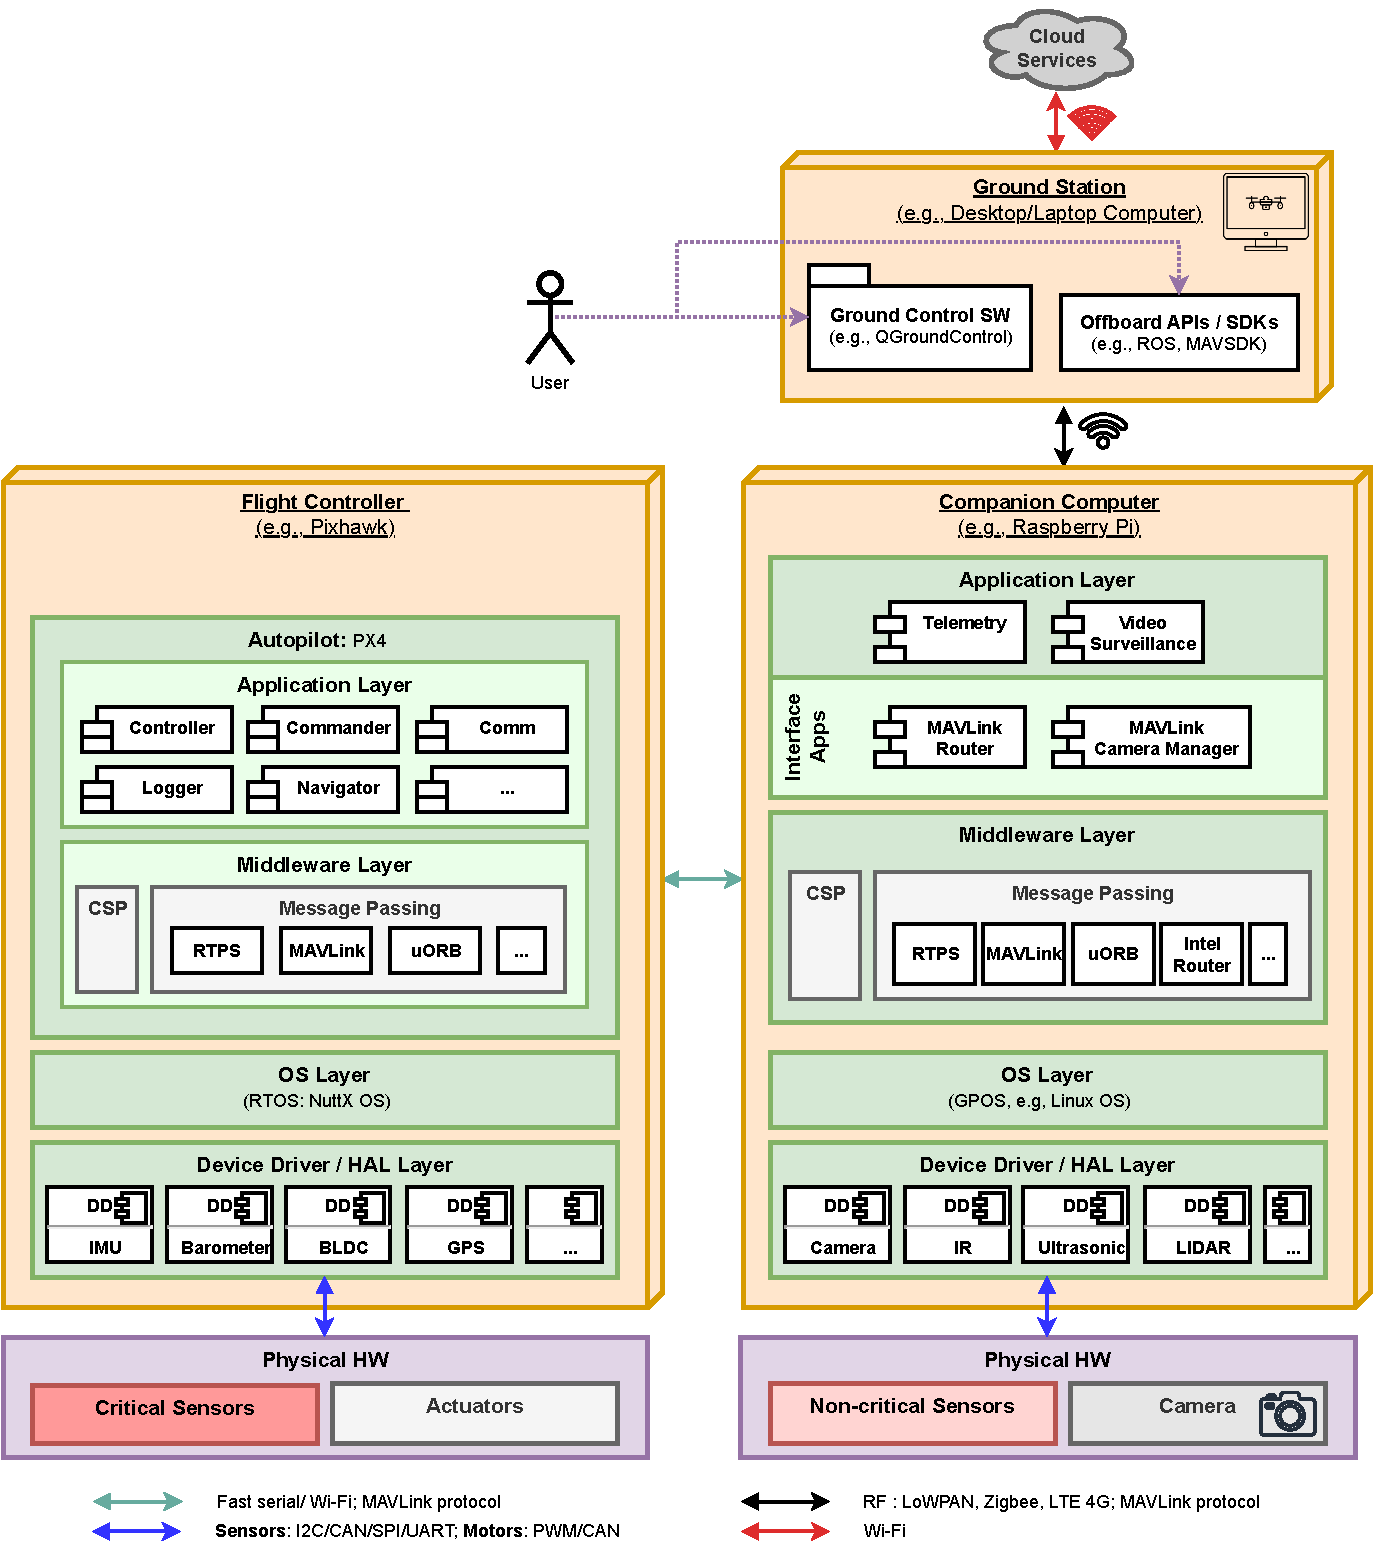
\includegraphics[width=1.0\textwidth]{./img/pdf/uav-main-design-conv-sol-1.pdf} 
%  \includesvg[width=1.0\textwidth]{./img/virtualization.svg} 
  %\caption[Virtualization mind map]{Virtualization mind map}%
  \caption{UAV design: conventional solution --- full}%
  \label{fig:uav-design-conv-sol-1}
\end{figure}

The PX4 flight controller stack was selected for this work due to its
open-source nature, extensive platform support, modular architecture, and
widespread adoption in the industry. PX4 runs on the flight controller on top of
the NuttX \gls{rtos}. In the generic case, the companion computer is used to
route communications between the \gls{gcs} and the \gls{fmu}: a fast serial
link, typically \gls{uart} or Ethernet, is established between the \gls{fmu} and
the companion computer using the MAVLink protocol; the companion computer
runs extra software to route the MAVLink traffic,
e.g. \href{https://github.com/mavlink-router/mavlink-router}{MAVLink
  Router}~\cite{px4-routers}.

The \texttt{User} interacts with the Ground Control \gls{sw}, namely
\texttt{QGroundControl}. \texttt{QGroundControl} was selected due to its
open-source nature and compatibility with the PX4 flight stack. Additionally,
the User can interact with the Companion Computer via offboard
\glspl{api}/\glspl{sdk}, e.g., \texttt{MAVSDK}. The \gls{rc} link was dropped,
as it is only usable in manual mode, thus, it is not useful for the video
surveillance application.

In the vast majority of cases, we also need extra software running on the companion
computer to interface the camera, e.g. the \href{https://github.com/mavlink/mavlink-camera-manager}{Mavlink Camera Manager}. This
component acts as bridge between the \gls{fmu} and \gls{gcs} and a translator between the MAVLink Camera Protocol v2
(used by PX4) and the native protocol of the camera~\cite{px4-cam-managers}.

The communications routing poses an increased risk to the \gls{uav}: if the
companion computer is compromised the \gls{fmu} may malfunction due to data
corruption or communication loss. Furthermore, the additional software required
to route MAVLink traffic and manage the camera adds complexity and latency to
the system.

Fig.~\ref{fig:uav-design-conv-sol-2} showcases a simplified conventional
solution customized for video surveillance, with a higher degree of
decoupling. Dedicated
communication links are established for communication between the \gls{gcs} and \gls{fmu} (telemetry radio) and the
camera (Wi-Fi). To streamline the network configuration and eliminate the need
for additional hardware, the \gls{gcs} and the \gls{uav} are integrated into the
same \gls{lan}. The video surveillance software is also simplified consisting of
a client running on the \gls{gcs} and the server running on the companion
computer supported by a suitable video pipeline and device drivers. The
client runs on port 5000 of the \gls{gcs} issuing command for the server running
on the same port in the Companion Computer. The server handles commands and
requests the sender to setup the video pipeline and transmit video frames back
to the \gls{gcs}. The receiver sets up a video pipeline on the \gls{gcs} (not
displayed) that processes the video frames and displays it to the \texttt{User}.

\begin{figure}[!hbt]
  \centering
  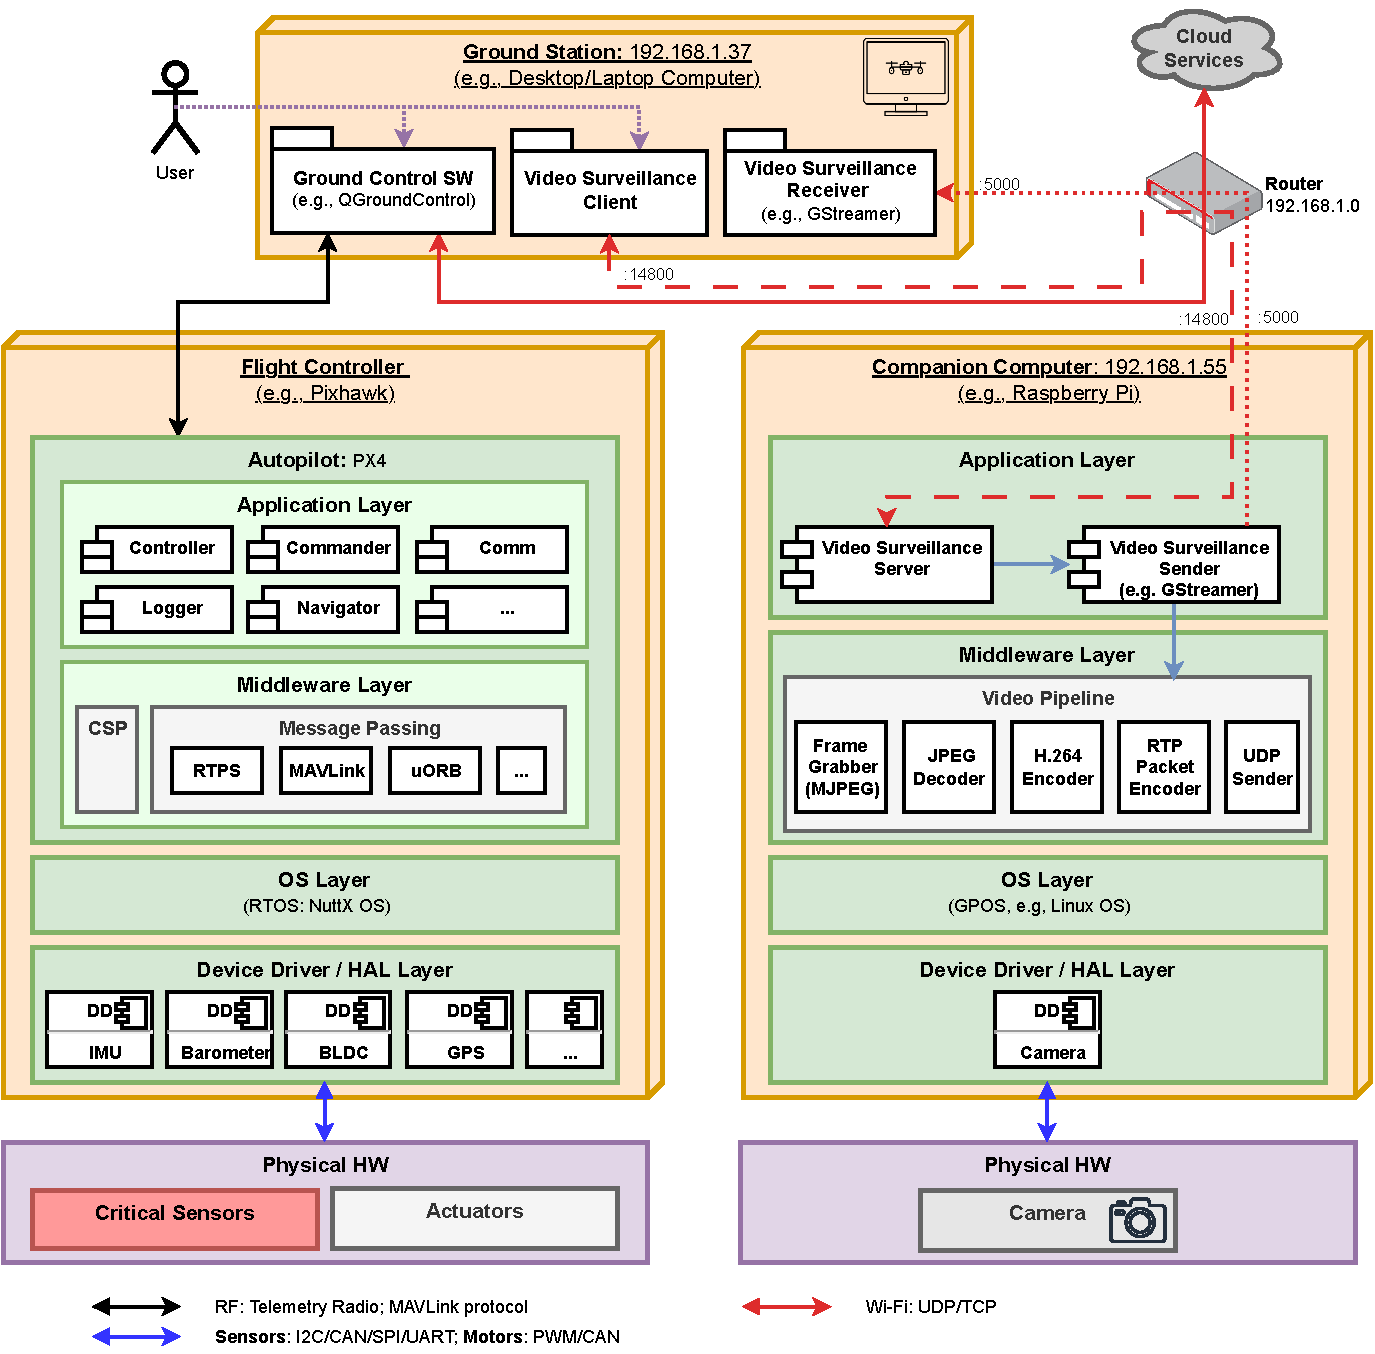
\includegraphics[width=1.0\textwidth]{./img/pdf/uav-main-design-conv-sol-2.pdf} 
%  \includesvg[width=1.0\textwidth]{./img/virtualization.svg} 
  %\caption[Virtualization mind map]{Virtualization mind map}%
  \caption{UAV design: conventional solution --- simplified}%
  \label{fig:uav-design-conv-sol-2}
\end{figure}

On the receiving end of the video surveillance system (\gls{gcs}), occasional frame loss is tolerable and does not compromise situational awareness of the target area. Consequently, a communication protocol without delivery guarantees, such as \gls{udp}, is appropriate.

This simplified conventional solution forms the base design for the platform
unification.

\subsection{Unsupervised Single-Platform Flight Stack}
\label{sec:unsuperv-stack}
To integrate the \gls{fmu} and companion computer platforms, we require a method to encapsulate their functionalities into standalone components within a unified platform. In the \glsxtrfull{uspfs}, these components are abstracted as processes running on a \gls{gpos}.

Fig.~\ref{fig:uav-design-unsup} illustrates the system architecture of the
\gls{uspfs}. The software processes for the \gls{gcs} and \gls{uavic} are shown
in blue. The \gls{uavic} consolidates the \gls{fmu} and companion computer nodes
into a single platform operating on a \gls{gpos}, specifically Linux. PX4
executes on core 0, while the remaining cores are allocated for the video
surveillance application.

\begin{figure}[!hbt]
  \centering
  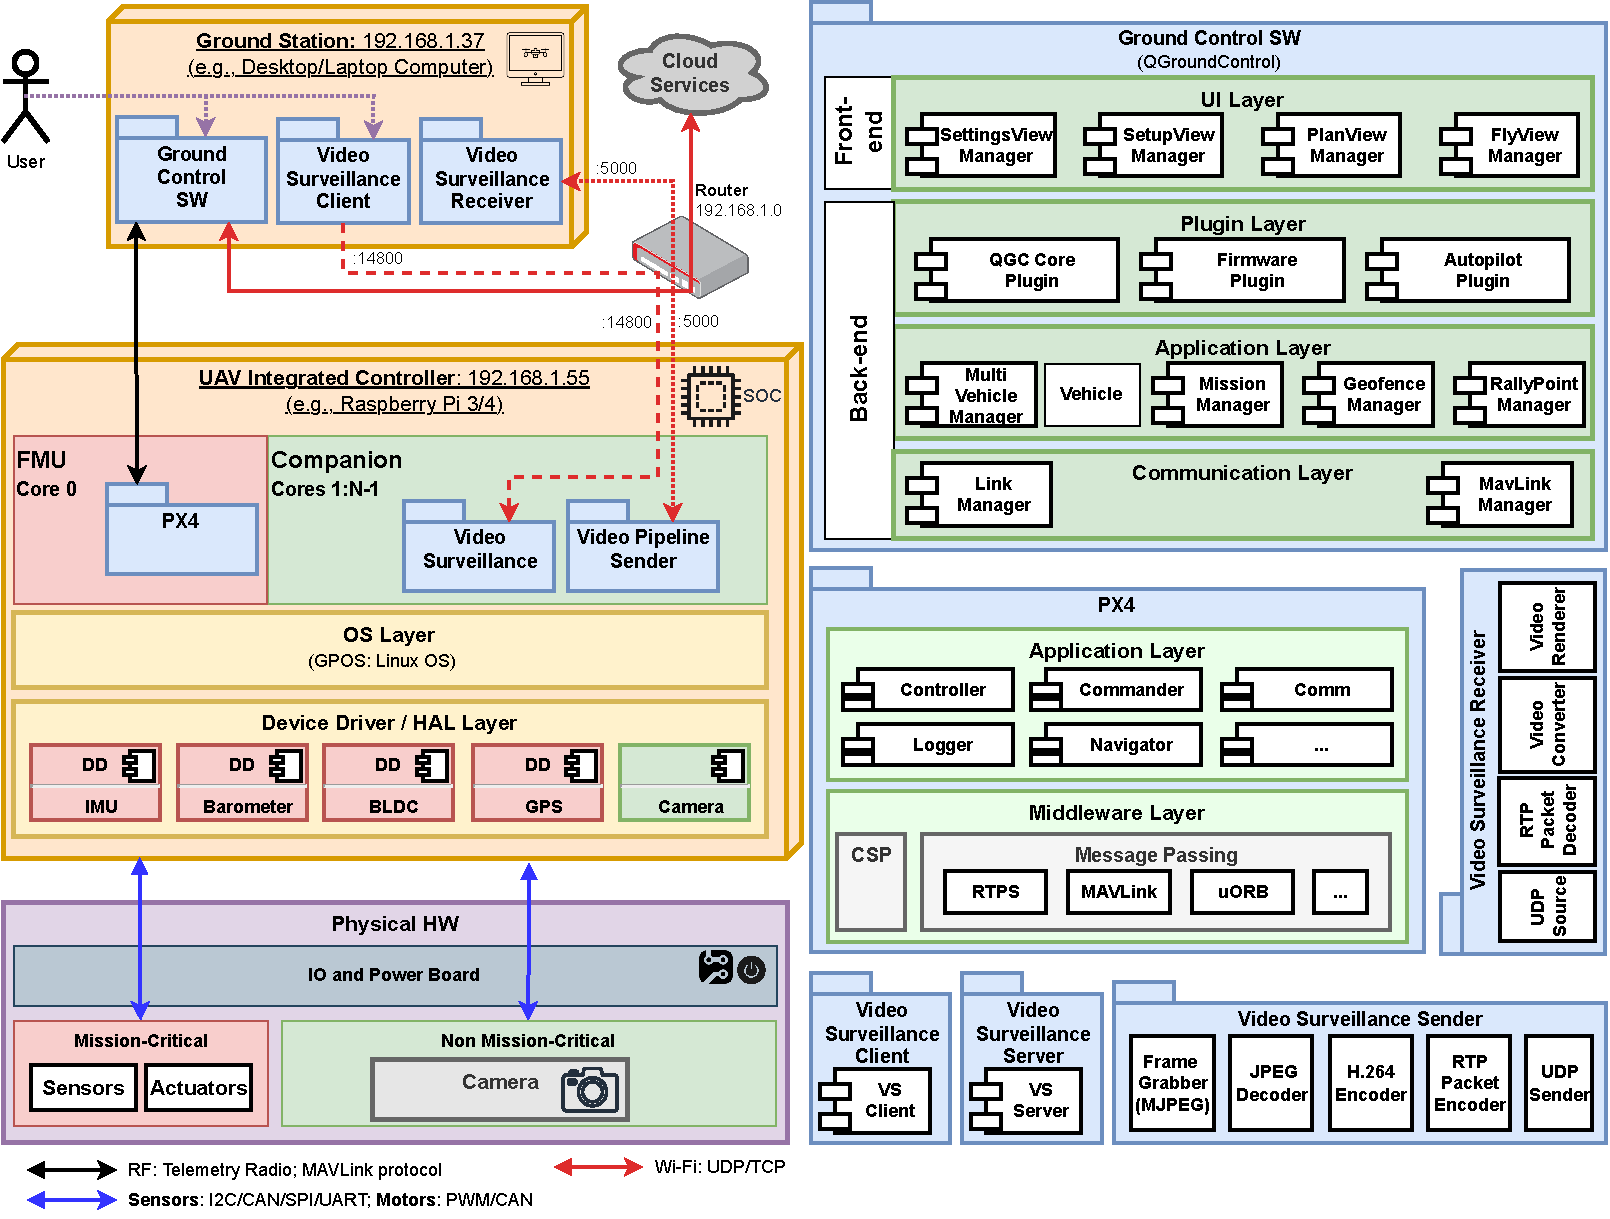
\includegraphics[width=1.0\textwidth]{./img/pdf/uav-main-design-unsup.pdf} 
%  \includesvg[width=1.0\textwidth]{./img/virtualization.svg} 
  %\caption[Virtualization mind map]{Virtualization mind map}%
  \caption{UAV design: Unsupervised Single-Platform Flight Stack}%
  \label{fig:uav-design-unsup}
\end{figure}

It is important to note that PX4 no longer runs on the Nuttx \gls{rtos}, which may introduce challenges in meeting the soft real-time requirements of flight control. To address this, one core is explicitly dedicated to the PX4 application. Additionally, employing a real-time Linux kernel with a suitable \gls{io} scheduler can help mitigate timing issues.

However, this architecture lacks isolation between systems, meaning a failure in the non-critical system can propagate to the \gls{fmu}. Such failures could lead to \gls{fmu} malfunctions, potentially resulting in a crash with unpredictable consequences. As mentioned earlier, this solution alone is insufficient; supervision is essential to ensure both reliable consolidation and safe integration.

\subsection{Supervised Single-Platform Flight Stack}
\label{sec:superv-stack}
Fig.~\ref{fig:uav-design-unsup} presents the system architecture of the
\glsxtrfull{sspfs}. In this design, the functionalities of the \gls{fmu} and
companion computer are abstracted as guest \glspl{vm} running atop the Bao
Hypervisor in the \gls{uavic} node. This approach ensures isolation between the two mixed-criticality
systems, preventing faults in the non-critical system from impacting the
\gls{fmu} and causing potential malfunctions.

\begin{figure}[!hbt]
  \centering
  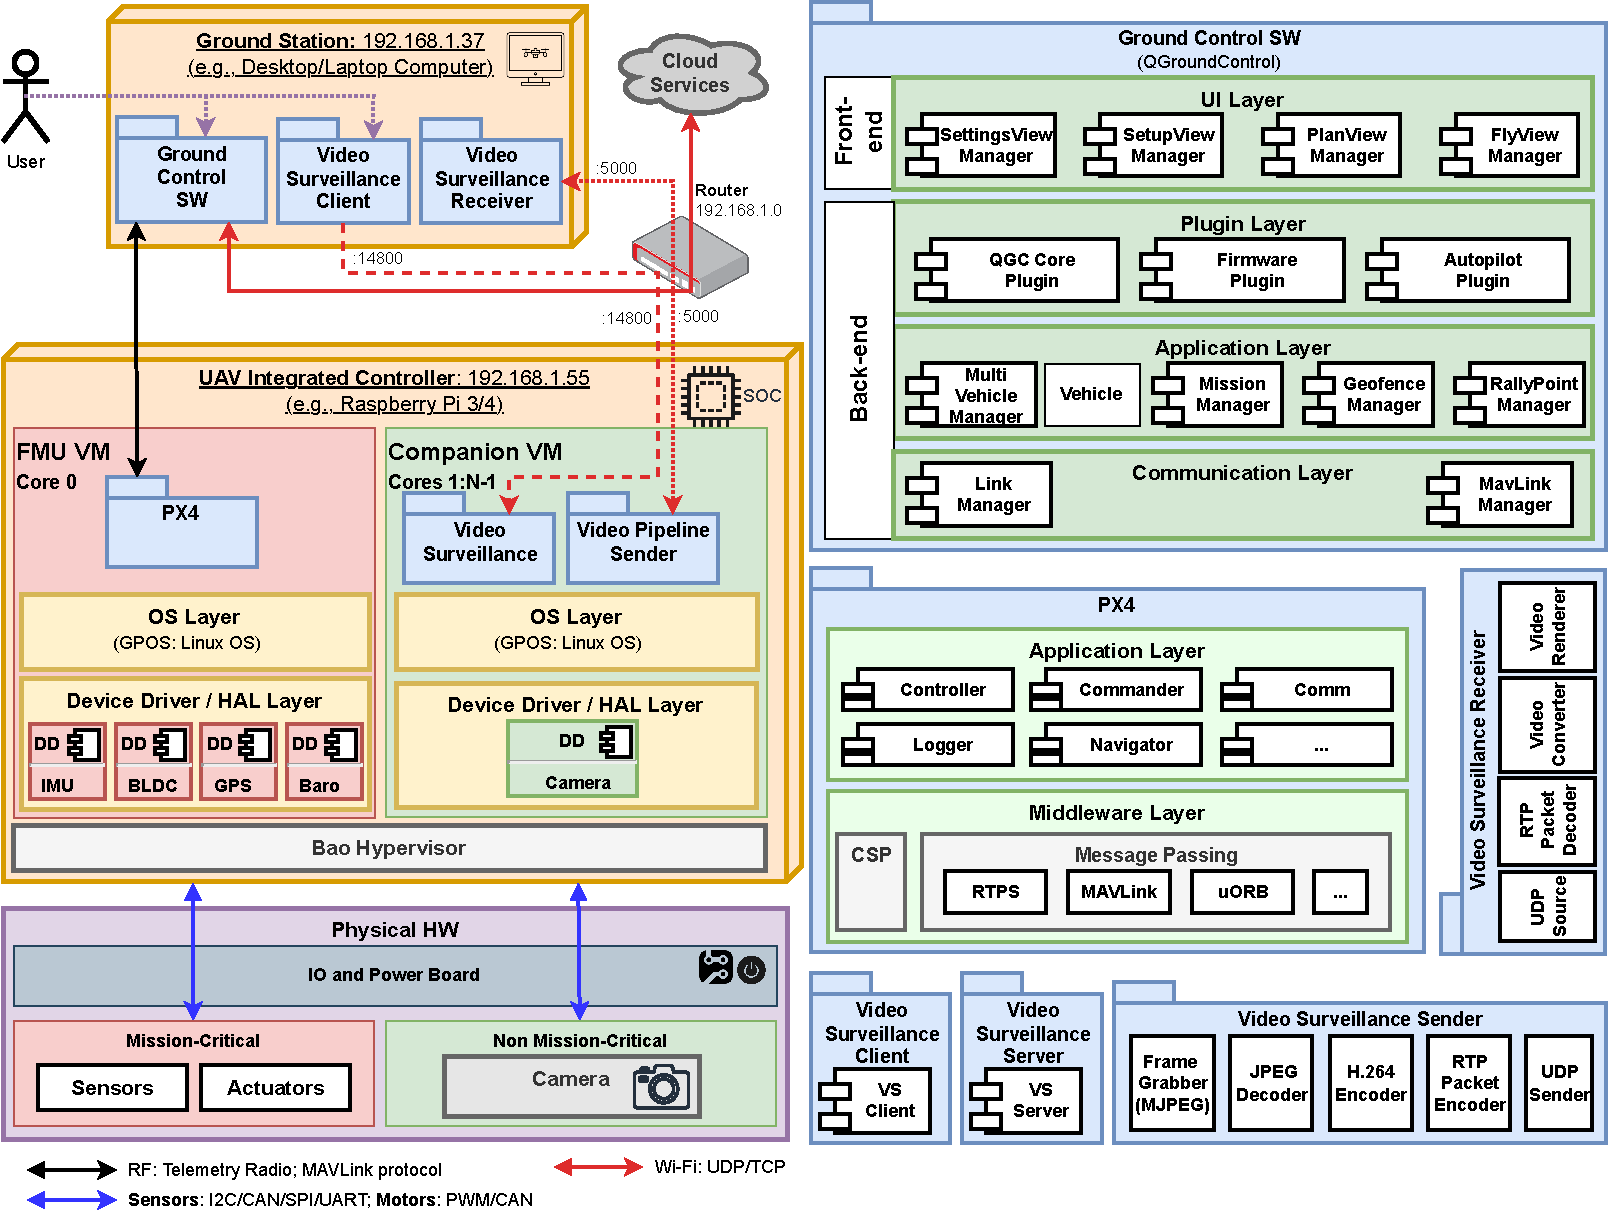
\includegraphics[width=1.0\textwidth]{./img/pdf/uav-main-design-sup.pdf} 
%  \includesvg[width=1.0\textwidth]{./img/virtualization.svg} 
  %\caption[Virtualization mind map]{Virtualization mind map}%
  \caption{UAV design: Supervised Single-Platform Flight Stack}%
  \label{fig:uav-design-sup}
\end{figure}

Each \gls{vm} operates a Linux-based \gls{os}, enabling further customization. For instance, the \gls{fmu} \gls{vm} can utilize a real-time kernel, providing additional guarantees that its assigned core remains fully dedicated to its execution. Meanwhile, the Companion \gls{vm} can operate with a standard Linux kernel. Bao's static partitioning mechanism guarantees that the hardware resources assigned to each \gls{vm} are strictly dedicated, ensuring isolation. Moreover, device drivers within each \gls{vm} are specific to that \gls{vm}, minimizing the impact of software bugs or failures.

However, this approach requires each \gls{vm} to include a full \gls{os},
leading to larger binary sizes. Additionally, the \texttt{User} must carefully
select and allocate hardware resources to avoid conflicts between \glspl{vm}
while maintaining adequate performance in terms of \gls{ram}, available
\glspl{cpu}, and other critical resources. This requires a deeper knowledge
about the hardware used. As such, we will later revisit the system architecture
to adapt it to the selected hardware.

\section{Hardware Selection}
\label{sec:hardware-selection}
In this section, the hardware for the \gls{uav}, \gls{uavic}, and
extra addons are selected. The hardware is mapped to comply with PX4
requirements and the \gls{uavic} restrictions imposed by Bao.

\subsection{UAV}
\label{sec:uav-hw-sel}
We will start by defining the \gls{uav}'s main characteristics. The multirotor
airframe was selected due to its low price and high availability, but especially
due to its compactness and \gls{vtol} support. It will be used in the \gls{lap}
altitude range (up to 3 to 9 kilometers). The \gls{uav} must be battery powered
and the overall weight must be small to extend battery life. Lastly, but most
importantly, it must be open-source to enable user's modification/customization. 

Fig.~\ref{fig:hoverGames-drone} shows the selected \gls{uav} --- the
\texttt{KIT-HGDRONEK66}, commonly referred to as the NXP HoverGames \gls{uav}
kit~\cite{nxp-hoverGames-uav}. This \gls{diy} professional development kit, priced under
500 USD, features the RDDRONE-FMUK66 as the \gls{fmu} unit (1).

\begin{figure}[!hbt]
  \centering
  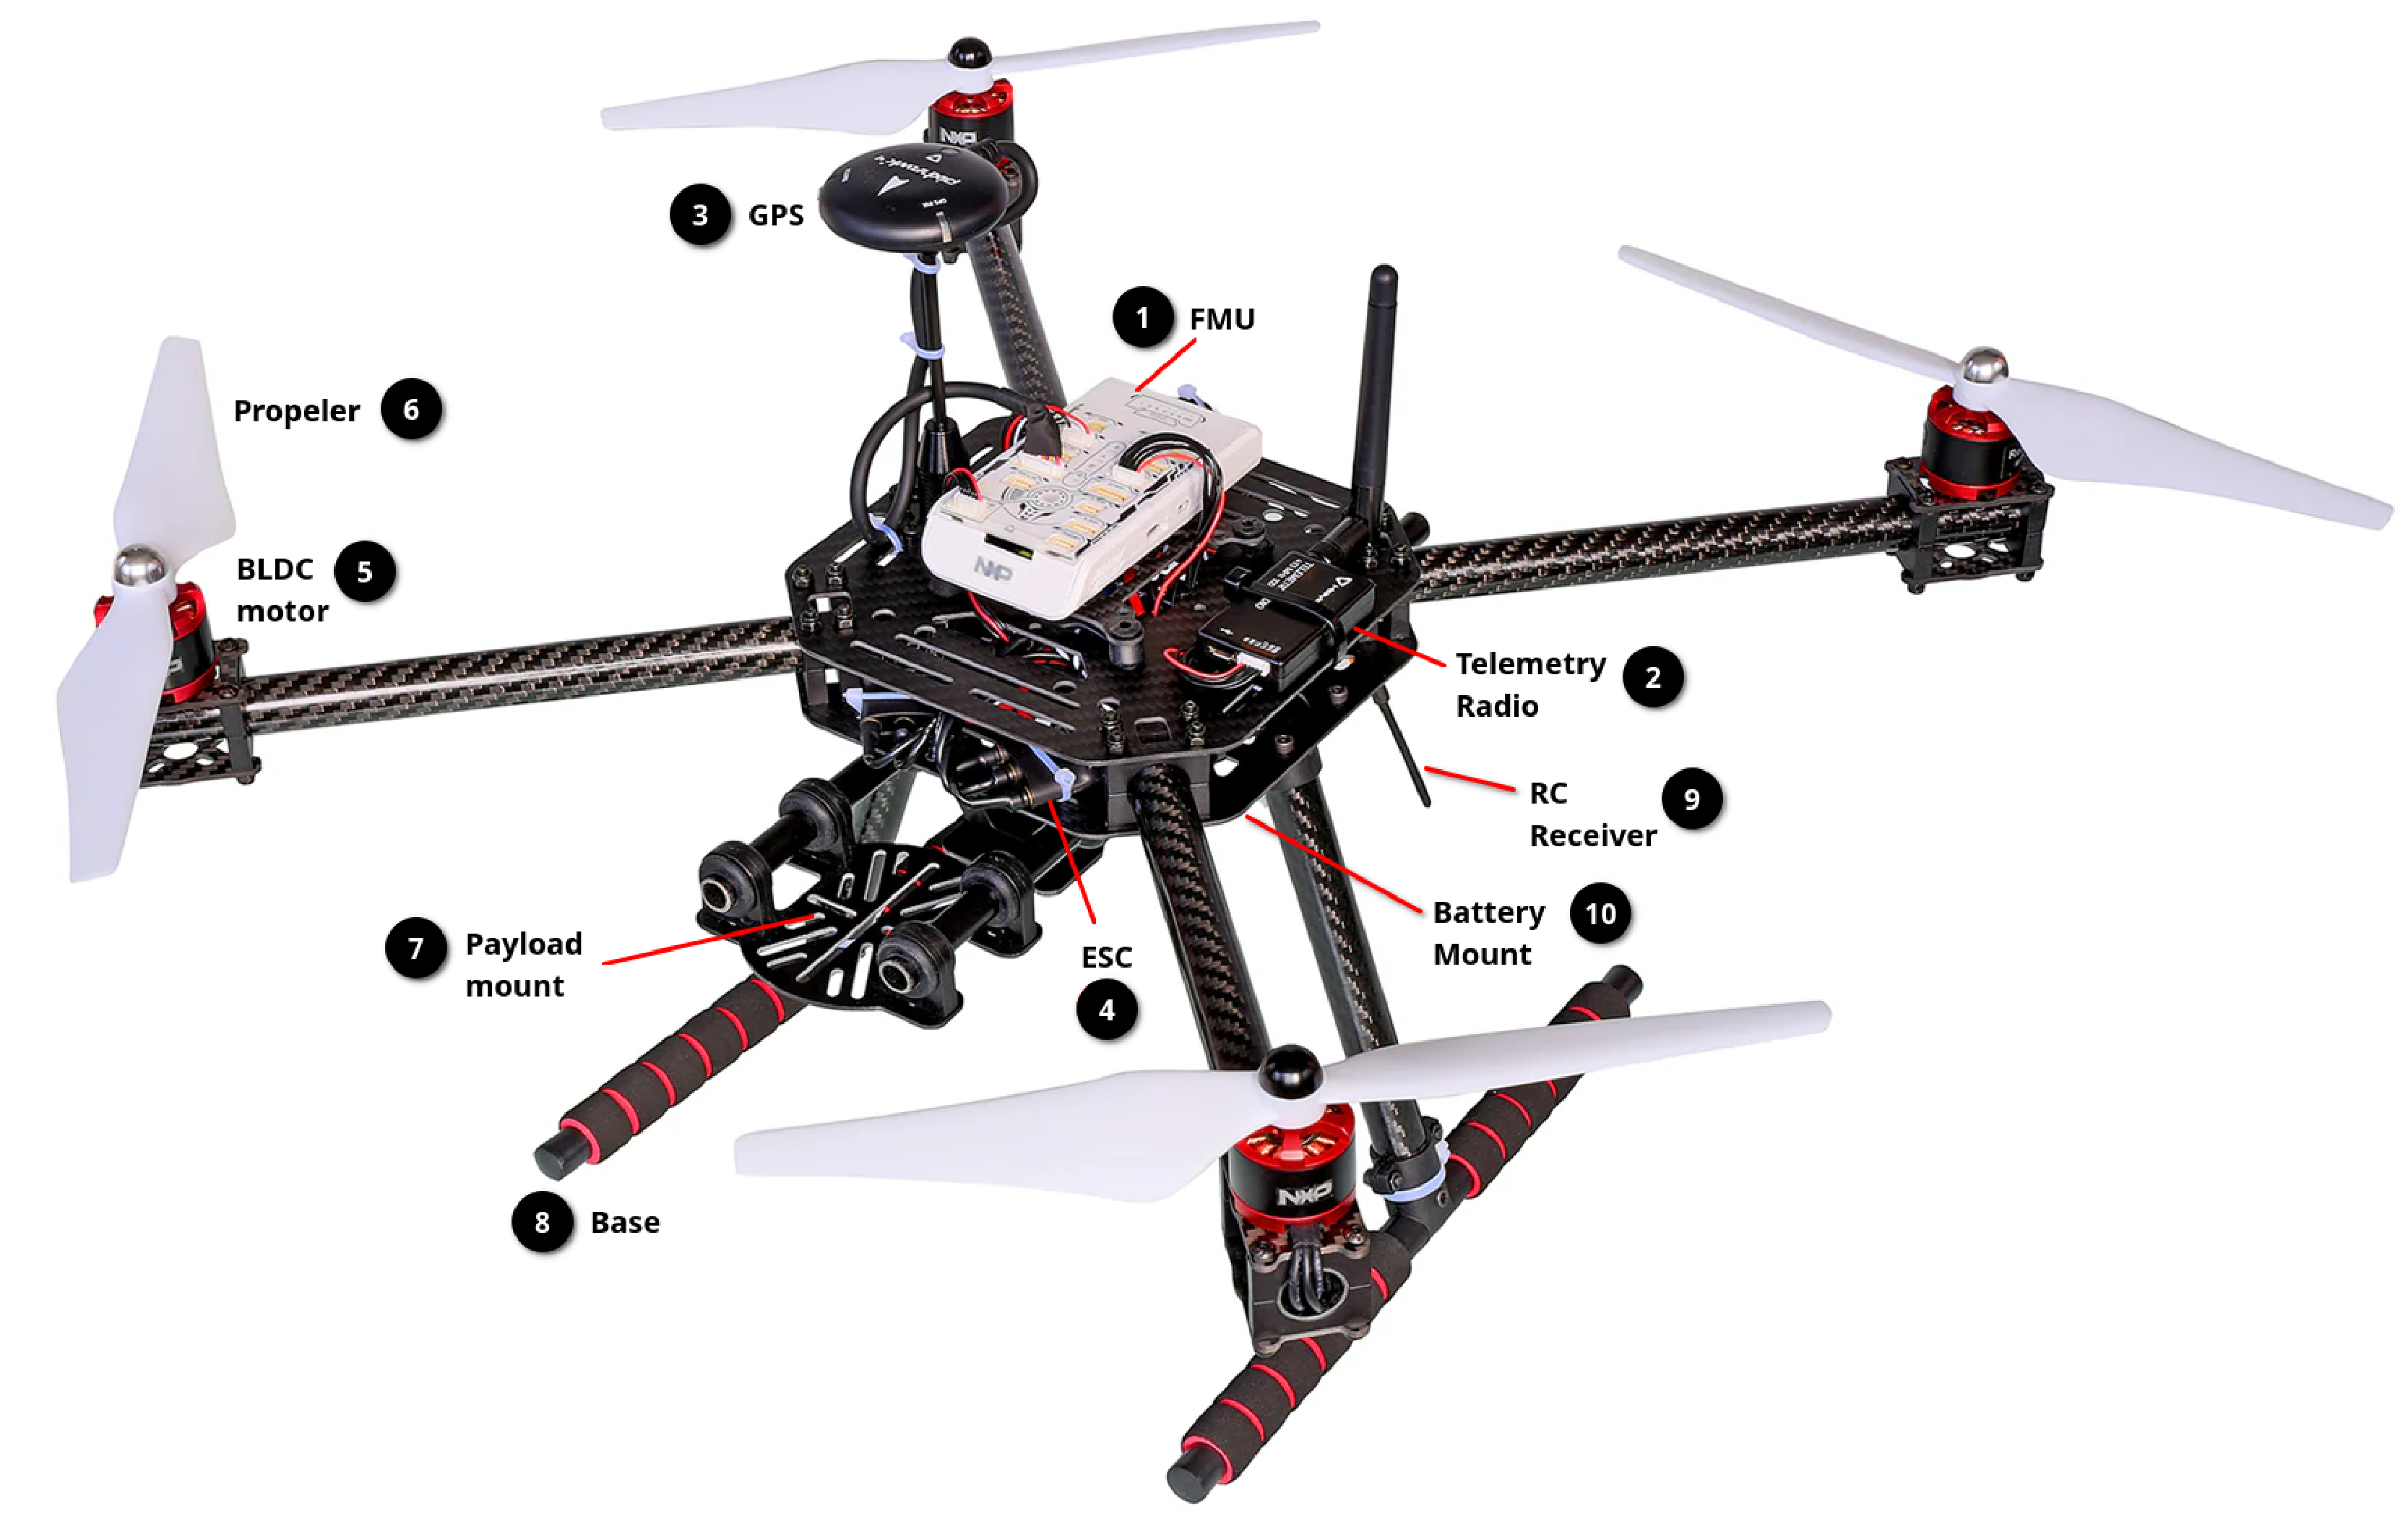
\includegraphics[width=1.0\textwidth]{./img/pdf/hoverGames-drone.pdf} 
  \caption[NXP HoverGames UAV kit]{NXP HoverGames UAV kit (adapted from~\cite{nxp-hoverGames-uav})\footnotemark}%
  \label{fig:hoverGames-drone}
\end{figure}
%
\fnlicNC{NXP Semiconductors}

The kit is built on an S500 carbon fiber frame with four rotors (quadcopter) and has a 500-millimeter wheelbase (diagonal distance between opposing motors). It employs \gls{bldc} motors (5) to drive the propellers (4), which are controlled by individual \gls{esc} units (4).

For autonomous flight capabilities, the kit includes a \gls{gps} module (3) and a payload mount (7) designed for accessories such as cameras. Power is supplied via a 3S \gls{lipo} battery (sold separately) with a capacity ranging from 3500 to 5000 mAh.

Additionally, a telemetry radio (2), also sold separately, can be connected to
the \gls{fmu} (1). This telemetry module operates in the 433 MHz frequency band
in Europe, enabling remote communication and monitoring.
%
The kit also includes the \gls{gps} NEO-M8N module and the \gls{rc} remote
controller GS-i6S transmitter and receiver modules.

Fig.~\ref{fig:hoverGames-blkDiag} depicts the block diagram for the NXP
HoverGames \gls{uav} kit.  It features the RDDRONE-FMUK66 \gls{fmu} using the
Kinetis\textreg K66 \gls{mcu} based on the 32-bit Arm\textreg
Cortex\textreg--M4 Core~\cite{nxp-hoverGames-fmu}, running at 180 MHz
with up to 2 MB of flash and 256 KB of \gls{sram}. The \gls{fmu} runs the PX4
autopilot stack.

\begin{figure}[!hbt]
  \centering
  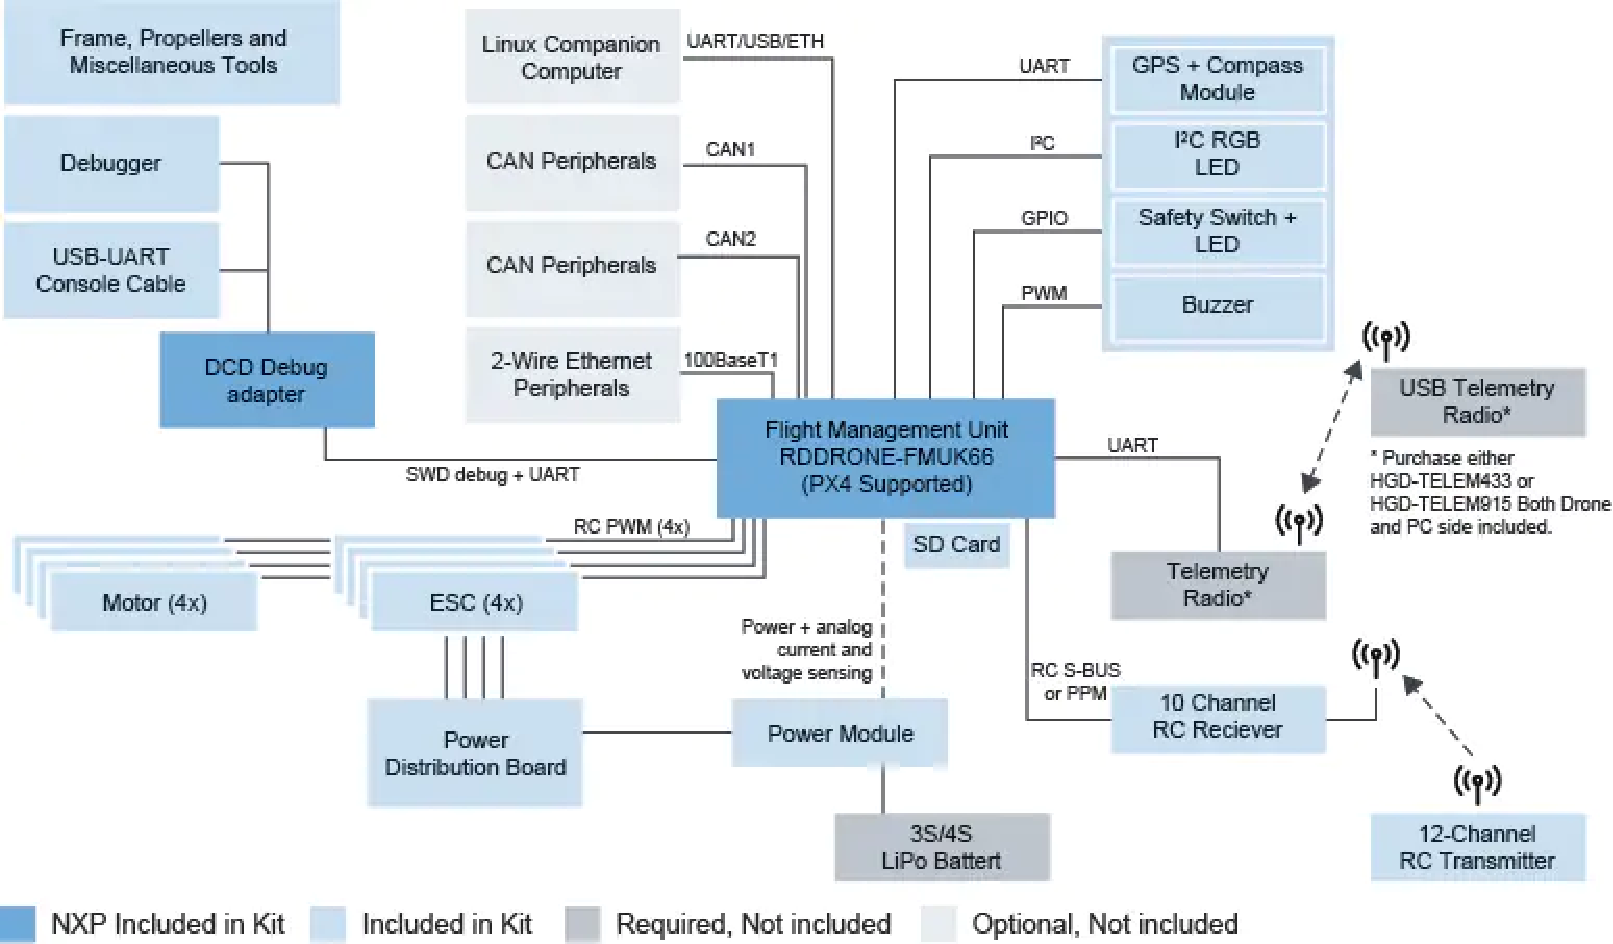
\includegraphics[width=1.0\textwidth]{./img/pdf/hoverGames-blkDiag.pdf} 
  \caption[NXP HoverGames block diagram]{NXP HoverGames block diagram (withdrawn from~\cite{nxp-hoverGames-uav})\footnotemark}%
  \label{fig:hoverGames-blkDiag}
\end{figure}
%
\fnlicNC{NXP Semiconductors}

It includes a power module and power distribution
board with current and voltage sensing to assess the \gls{uav}'s \gls{lipo}
battery autonomy. The power distribution board supplies the \gls{bldc} motors,
controlled by the \gls{esc} unit using \gls{pwm}. A SEGGER J-Link EDU Mini \gls{swd} adapter can
be used to debug the running flight stack or to upload it to the \gls{fmu}. 

It supports common \gls{uav} sensors such as accelerometer, gyrometer,
magnometer, compass, and barometer.
The \gls{fmu} can communicate with a companion computer via \gls{uart}, or with
the \gls{gcs} via the telemetry radio or \gls{rc} link. An optional \gls{sd}
card can be used to support flight logging for offline analysis, debug, and
replay in simulation tools.

\subsection{UAV Integrated Controller}
\label{sec:uav-integr-contr}
The \glsxtrfull{uavic} merges the \gls{fmu} and companion computer functionalities
into a single platform. To achieve this, we deploy the PX4 autopilot stack and
the video surveillance application into a custom Linux-based OS. However, PX4 was
typically designed to run atop of the NuttX \gls{rtos} and the support for Linux
is fairly limited. The supported platforms include the BeagleBone Blue and the
Raspberry Pi 2/3/4 with additional
shields~\cite{px4-experimental-autopilot}. 

Fig.~\ref{fig:pilotpi-annot} presents the chosen \gls{uavic}, the Raspberry Pi
4 with the PilotPi shield, due to its detailed documentation and lower
cost. The PilotPi shield is a fully functional and open-source solution to run
the PX4 autopilot directly on the Raspberry Pi. No proprietary driver is
required and \gls{pcb} and schematic are open source as well~\cite{px4-pilotpi}.

\begin{figure}[!hbt]
  \centering
  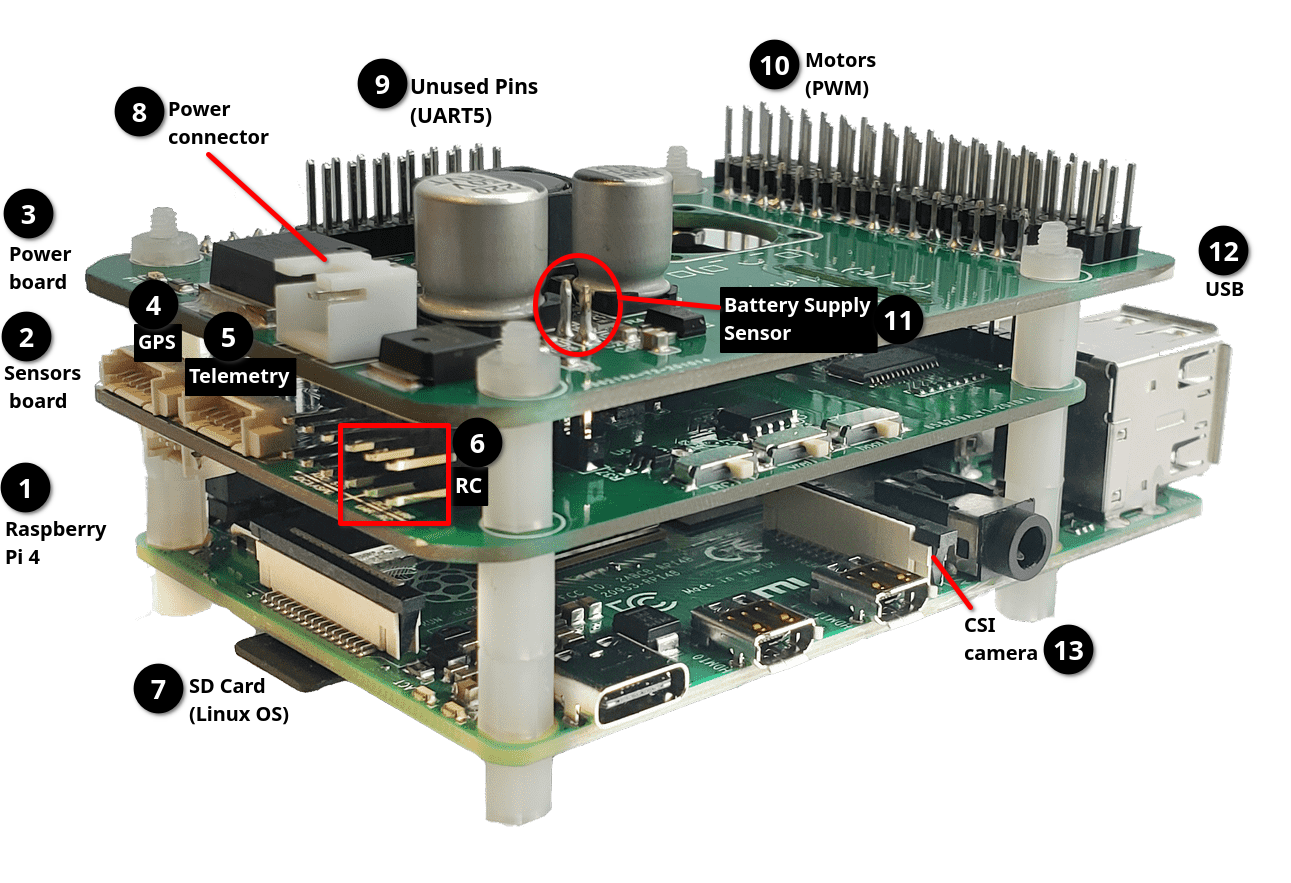
\includegraphics[width=1.0\textwidth]{./img/png/pilotpi-annotated} 
  \caption[UAVIC: Raspberry Pi 4 + PilotPi shield]{UAVIC: Raspberry Pi 4 +
    PilotPi shield (adapted from~\cite{px4-pilotpi}\footnotemark}%
  \label{fig:pilotpi-annot}
\end{figure}
%
%\fnlicReq{Elsevier}{5457890117132}%
\fnlicCCFour{foot:pilotpi-annotated}%

The Raspberry Pi 4 Model B (1) runs a Linux-based \gls{os}
from the \gls{sd} card and directly exposes the \gls{csi} camera and the
\gls{usb} interface. The Raspberry Pi 4 Model B features the Broadcom BCM2711
\gls{soc}, containing a 64-bit quad-core Arm\textreg Cortex\textreg--A72 \gls{cpu} running
at up to 1.8 GHz and a VideoCore VI \gls{gpu} running at up to 500
MHz~\cite{rpi4-specs,rpi4-bcm2711}, with 8 GB LPDDR4-3200 SDRAM. It provides 2.4
and 5.0 GHz 802.11ac wireless, Bluetooth 5.0, Gigabit Ethernet, and two
\gls{usb} 3.0 and two \gls{usb} 2.0 ports.

On top of the Raspberry Pi we have the sensors board (2),
providing \gls{gps}, telemetry and \gls{rc} external interfaces, mapped to
\texttt{/dev/ttySC0}, \texttt{/dev/ttySC1}, and \texttt{/dev/ttyAMA0},
respectively. Additionally, it provides onboard accelerometer/gyroscope
(\texttt{ICM42688P}), magnetometer (\texttt{IST8310}), and barometer
(\texttt{MS5611}) sensors required by PX4.

Lastly, on the topmost
plane we have the power board (3) handling power supply (8) and monitoring (11)
and the motors actuation using \gls{pwm} (10) supported by the Linux's \texttt{PCA9685}
device driver. Additionally, it contains a
header exposing unused pins which can be used, for example, to establish a
remote serial connection (UART5).

\subsection{Hardware mapping}
\label{sec:hardware-mapping}
The \gls{uavic} platform must comply with PX4 requirements on the available
sensors and actuators. Furthermore, due to the static partitioning nature of the
Bao hypervisor it is important to assess in the \gls{sspfs} solution if the \gls{uavic} hardware is fully
available to each one of the guests, or if an alternative must be
provided. Thus, in this section, we will start by mapping the hardware required
by PX4 to the Linux device tree for the \gls{uspfs} solution. Then, we will
adapt it to comply with Bao constraints in the \gls{sspfs} solution.


\subsubsection{USPFS}
\label{sec:base-scenario}
Fig.~\ref{fig:hw-map-1} depicts the full device tree for the \gls{uavic} system,
representing the \gls{uspfs} solution (base scenario).
The solid lines represent aggregation, i.e., a node that includes another one
(e.g., the \texttt{root} node includes the \texttt{memory} node), and the
dashed lines represent dependency, i.e., a node that depends on another one
(e.g., the \texttt{power} and \texttt{firmware} nodes depend on the
\texttt{mailbox}).

\begin{figure}[!hbt]
  \centering
  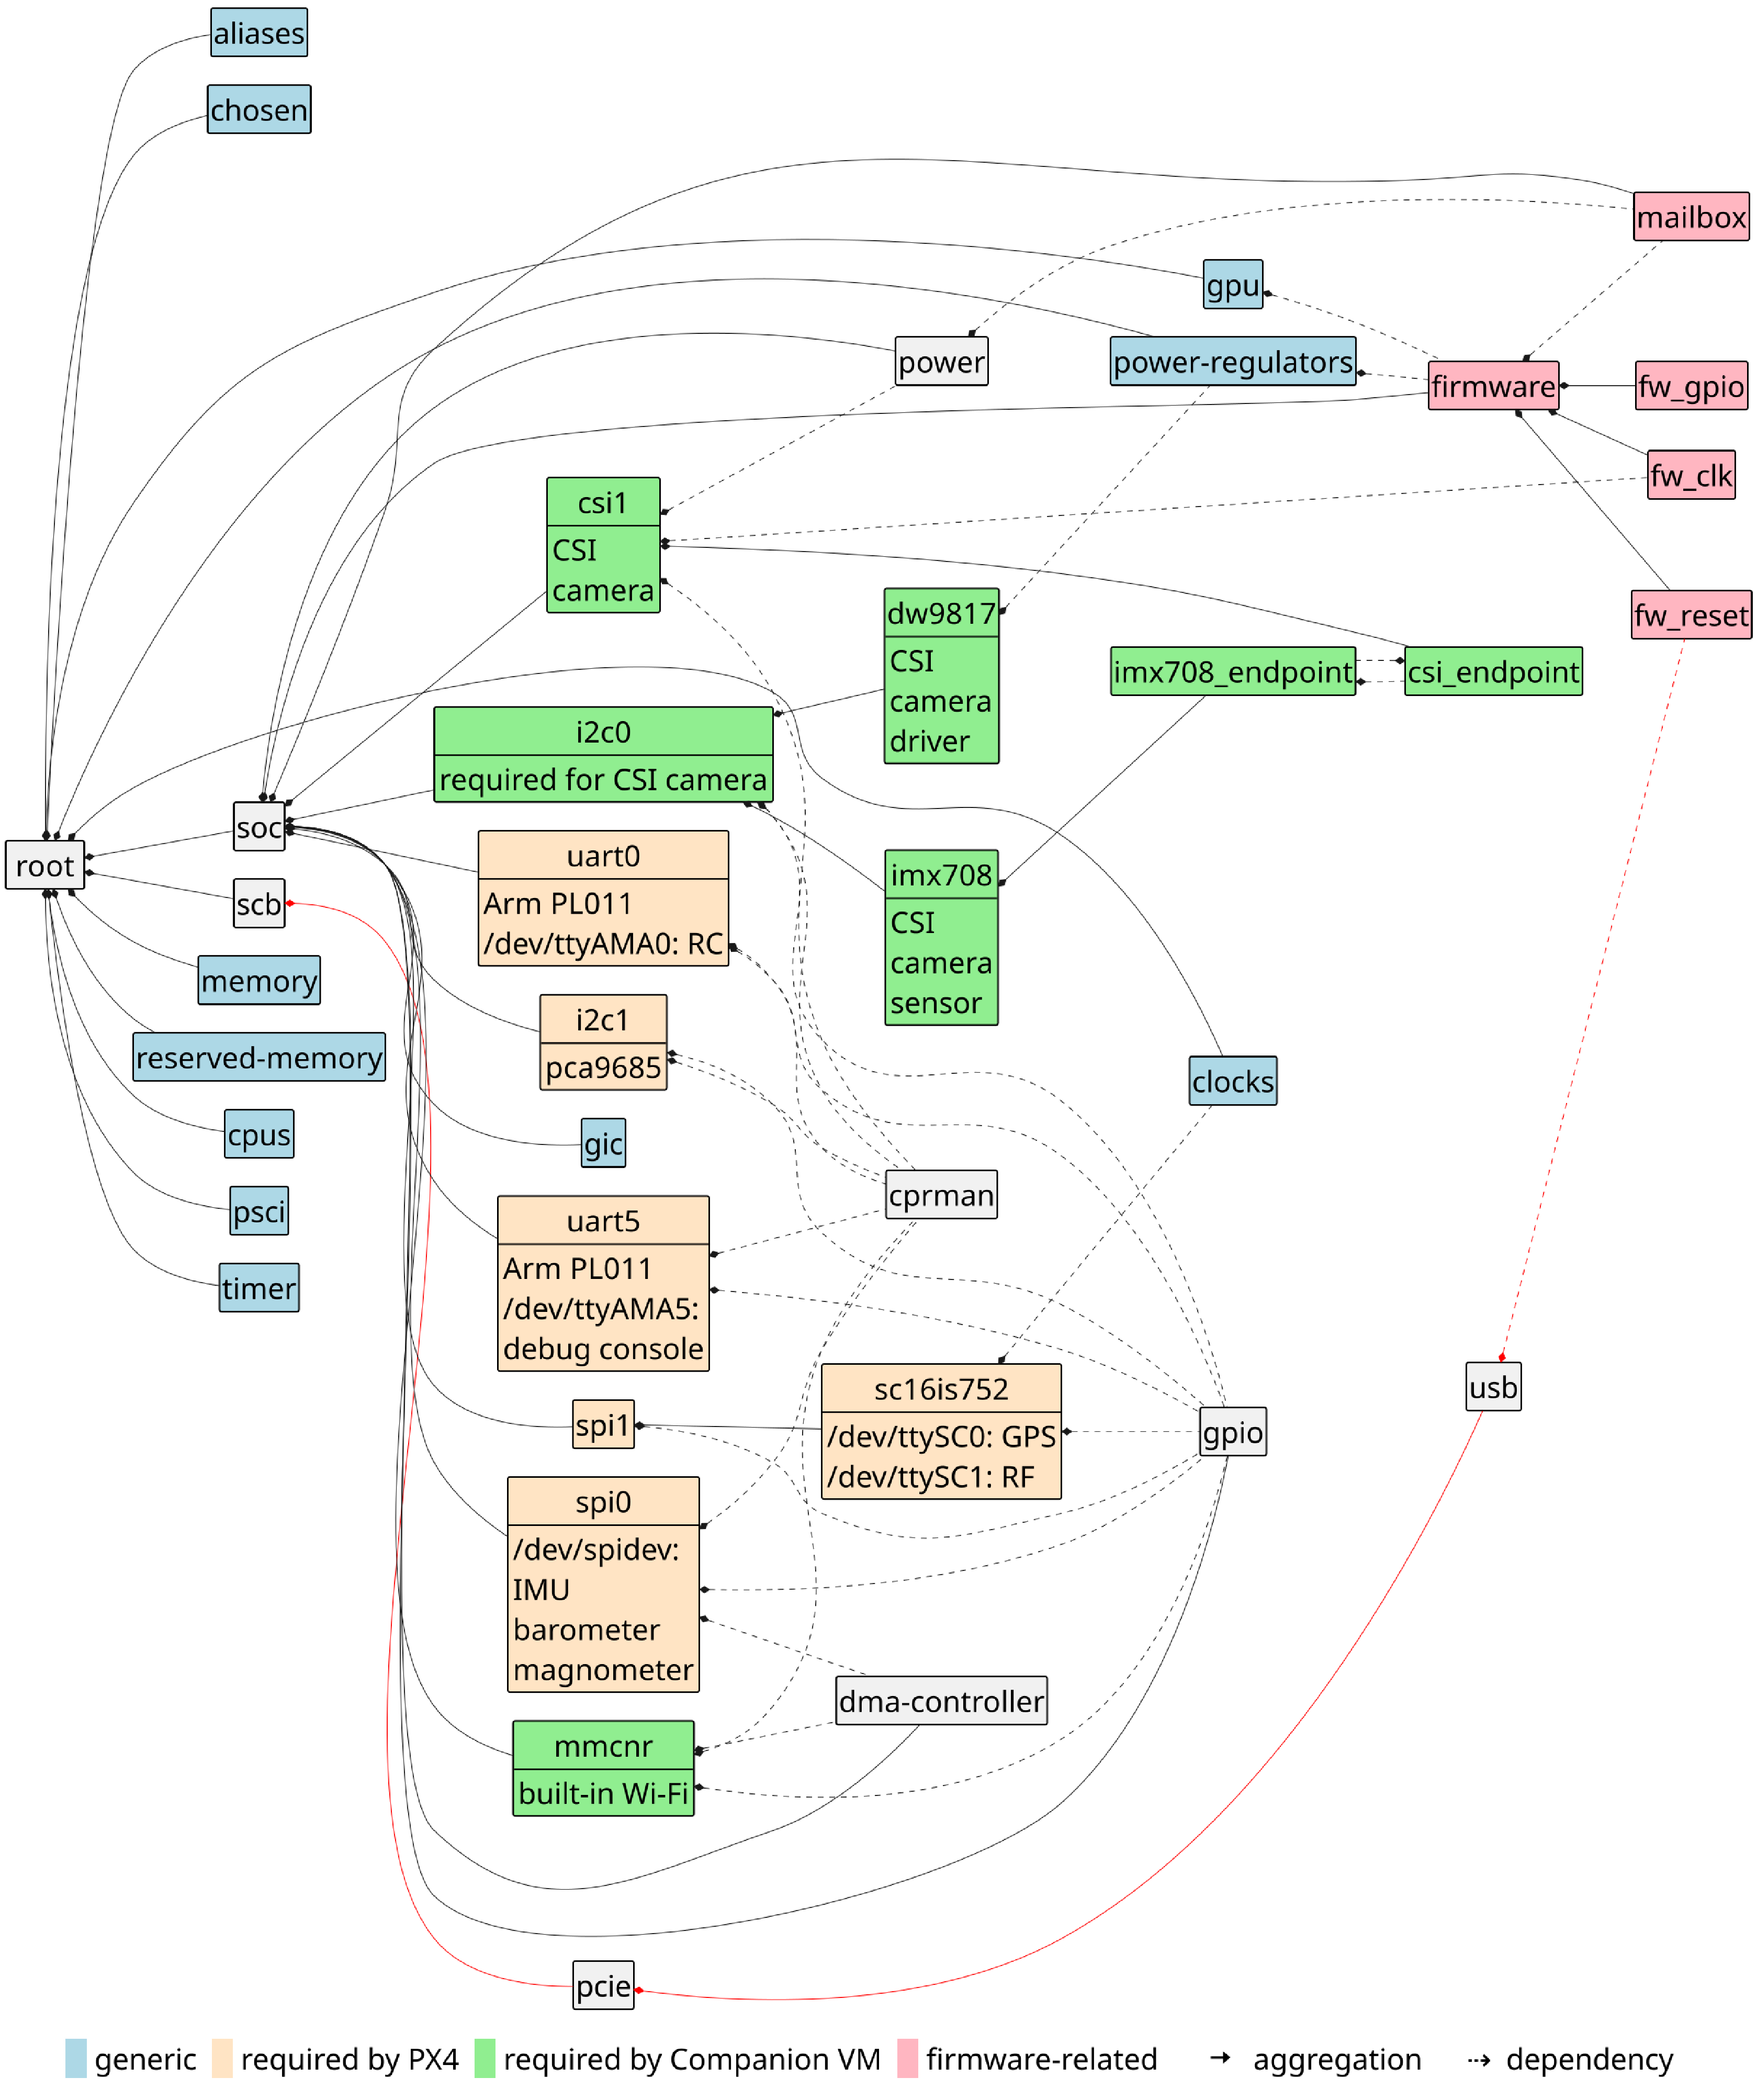
\includegraphics[width=1.0\textwidth]{./img/pdf/hw-map-1} 
  \caption[Hardware mapping: USPFS device tree]{Hardware mapping: \gls{uspfs}
  device tree}%
  \label{fig:hw-map-1}
\end{figure}

% \hexcolor{FFE4C4}{Bisque}
% \hexcolor{ADD8E6}{LightBlue}
% \hexcolor{90EE90}{LightGreen}
% \hexcolor{FFB6C1}{LightPink}
% \hlighthex{FFE4C4}{000000}{Bisque}
% \hlighthex{ADD8E6}{000000}{LightBlue}
% \hlighthex{90EE90}{000000}{LightGreen}
% \hlighthex{FFB6C1}{000000}{LightPink}

In \hlighthex{ADD8E6}{000000}{blue} we have the generic nodes that must be included in every device tree
version for the Raspberry Pi 4, e.g., \texttt{memory}, \texttt{cpus},
\texttt{power-regulators}, etc.. 
In \hlighthex{FFE4C4}{000000}{orange} we have the nodes required by
PX4: \texttt{i2c1} for the motors actuation, \texttt{spi0} for the \gls{imu},
barometer and magnometer, \texttt{spi1} for the \gls{gps} and the telemetry
radio, and \glspl{uart} 0 and 5 for \gls{rc} link and debug console,
respectively.
In \hlighthex{90EE90}{000000}{green} we have the nodes required by the companion
\gls{vm}, namely \texttt{i2c0} and \texttt{csi1} for the \gls{csi} camera, and
\texttt{mmcnr} to utilize the onboard Wi-Fi.
Lastly, in \hlighthex{FFB6C1}{000000}{pink} we have the firmware-related nodes,
which are used by the Rasbperry Pi \gls{gpu} to communicate with the Arm
\glspl{cpu} using the \texttt{mailbox}~\cite{rpi4-fw-mbox}.

Analyzing the device tree we can observe multiple common dependencies for PX4
and the Companion \gls{vm}: the clock manager \texttt{cprman}, the
\gls{gpio} controller, and the \gls{dma} controller. However, Bao disallows the
sharing of devices to ensure isolation between guests. As such, an alternative
must be provided to support PX4 and the Companion \gls{vm} in Bao.

One such alternative consists in maintaining PX4 as is, since it requires the
on-board sensors and has a larger number of devices, and migrating the Companion
\gls{vm}'s devices to the \gls{usb} interface. Following the
\textcolor{red}{red line}, we can verify that the \texttt{usb} device,
contained in the \texttt{pcie}, has only a common dependency with \texttt{PX4}
--- the \texttt{firmware} node --- which in turn depends on the
\texttt{mailbox}.

This is the simplest and most straightforward method to provide support for the
\gls{sspfs} solution. However, this still causes issues with Bao due to the
common \texttt{mailbox} node required by the \texttt{firmware}. On the other
hand, removing the \texttt{firmware} node from one of the \glspl{vm} is not an
option: doing so will lead to \gls{vm} malfunction.

Thus, the plan consists in migrating the Companion \gls{vm}'s devices to the
\gls{usb} interface and providing support in Bao to manage the access to the
shared mailbox in a supervised and secure form.

\subsubsection{Supervised mailbox access}
\label{sec:superv-mailb-access}
Fig.~\ref{fig:design-mailbox} illustrates the mailbox access for the
conventional case (left) and the supervised one (right).

\begin{figure}[!hbt]
  \centering
  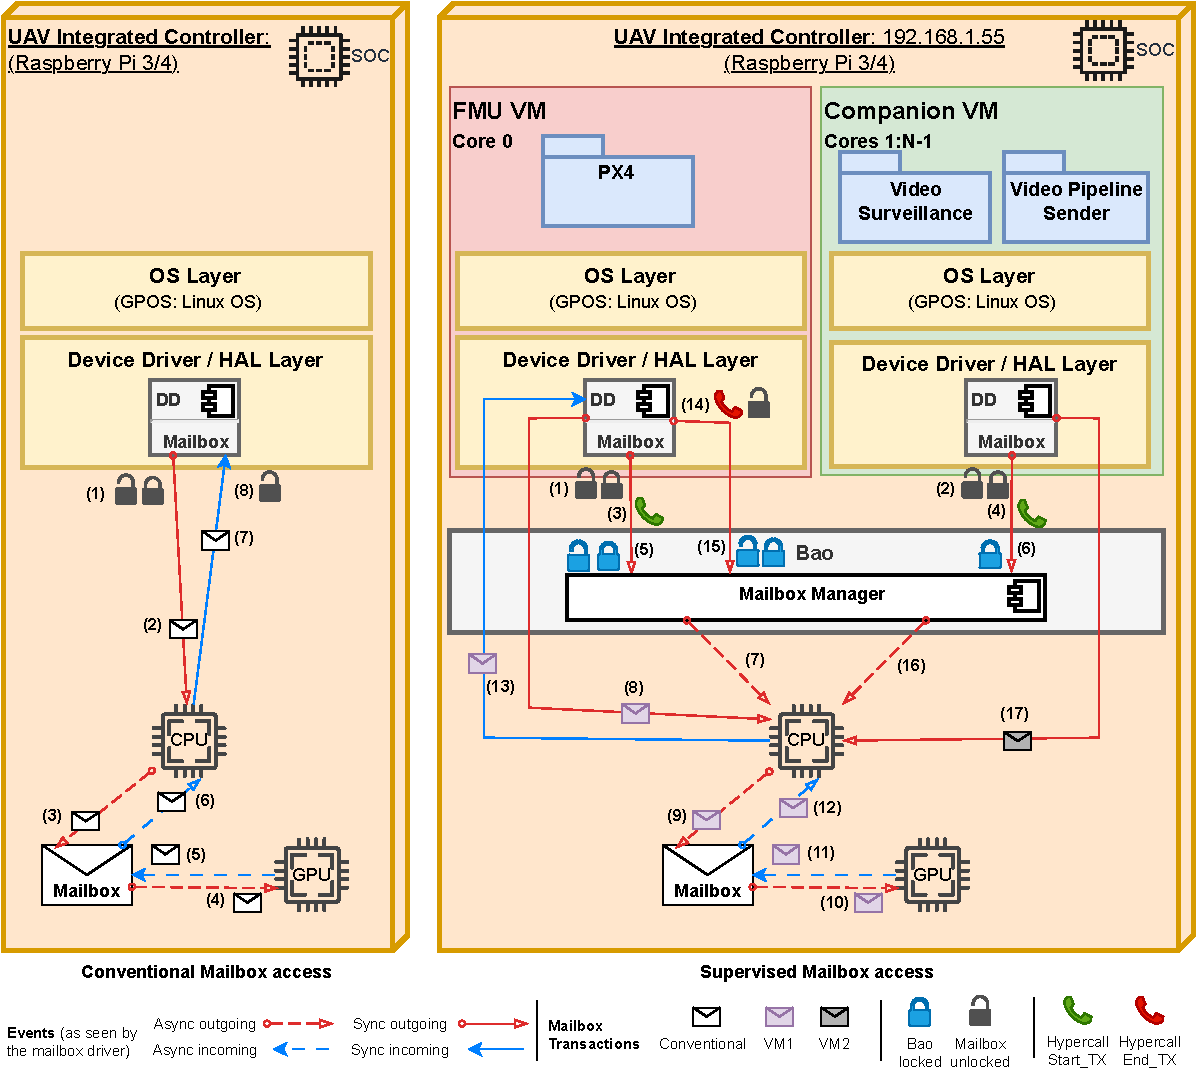
\includegraphics[width=1.0\textwidth]{./img/pdf/uav-main-design-mailbox} 
  \caption{Mailbox access: conventional (left); supervised (right)}%
  \label{fig:design-mailbox}
\end{figure}

The solid lines
indicate synchronous events, while the dashed ones
indicate asynchronous events, with the \textcolor{red}{red} arrows for the
outgoing path as seen by the mailbox driver and the \textcolor{blue}{blue} ones for the
incoming path. The mailbox transactions are represented with white, violet and
grey envelopes for the conventional, VM1 and VM2 interactions. The
synchronization mechanism (lock) is drawn in brown for the mailbox and in blue
for Bao. Hypercalls are represented with a green phone for \texttt{Start\_TX}
hypercall and a red one the \texttt{End\_TX} hypercall. Lastly, the numbering
indicates the sequence of events for both cases.

In the \textbf{conventional case}, the mailbox device driver can initiate a transaction
request if another transaction is not pending complete (1). The transaction must
be completed (8) before a timeout occurs, freeing the mailbox for further
requests. An interrupt is triggered (2) and the \gls{cpu} forwards the request
to the mailbox (3) which requests data from the \gls{gpu} (4). The \gls{gpu}'s
firmware handles the transaction and replies back to the mailbox with the
result (5). The mailbox forwards the response to the mailbox (6, 7) completing
the request and freeing the mailbox~\cite{rpi4-mbox-driver}. 

In the \textbf{supervised case}, the VM1 mailbox driver tries to initiate a
transaction request if another transaction is not pending complete (1). Now,
before sending the transaction, the mailbox driver must signal to Bao it wants
to start it by performing a \texttt{Start\_TX} hypercall (3). Bao acknowledges
this request if another one is not pending complete, locking the mailbox manager
(5). VM2 tries to do the same (2, 4), but, as VM1 acquired the lock, it must
wait for VM1 transaction completion. The Mailbox Manager handles the hypercall,
identifying the guest, the target device address (mailbox), and the interrupt
ID, and injecting the interrupt in the appropriate \gls{cpu} (7). The mailbox
device driver can now send the transaction to the mailbox (8, 9) which will
dispatch it to the \gls{gpu} (10). The \gls{gpu} processes the transaction and
the response it sent back to the device mailbox driver (11, 12, 13). When the
transaction is completed the mailbox driver issues another hypercall ---
\texttt{End\_TX} --- to signal Bao this event, and the mailbox lock is released,
freeing the VM1's mailbox for further requests. Bao handles the hypercall
\texttt{End\_TX} by releasing the mailbox manager's lock (15), which triggers
the pending transaction request issued by VM2 (6) to be resumed by injecting the
interrupt in the appropriate \gls{cpu} (16). Then, the VM2 mailbox's driver can
send the firmware transaction and the process continues.

\subsubsection{SSPFS}
\label{sec:final-scenario}
After addressing the shared device between \glspl{vm}, through the appropriate
supervision of the firmware's mailbox, we can now assign the available hardware
to each \gls{vm}.

Fig.~\ref{fig:hw-map-2} and Fig.~\ref{fig:hw-map-3} illustrates the device trees
for the PX4 \gls{vm} and Companion \gls{vm}, respectively.

\begin{figure}[!hbt]
  \centering
  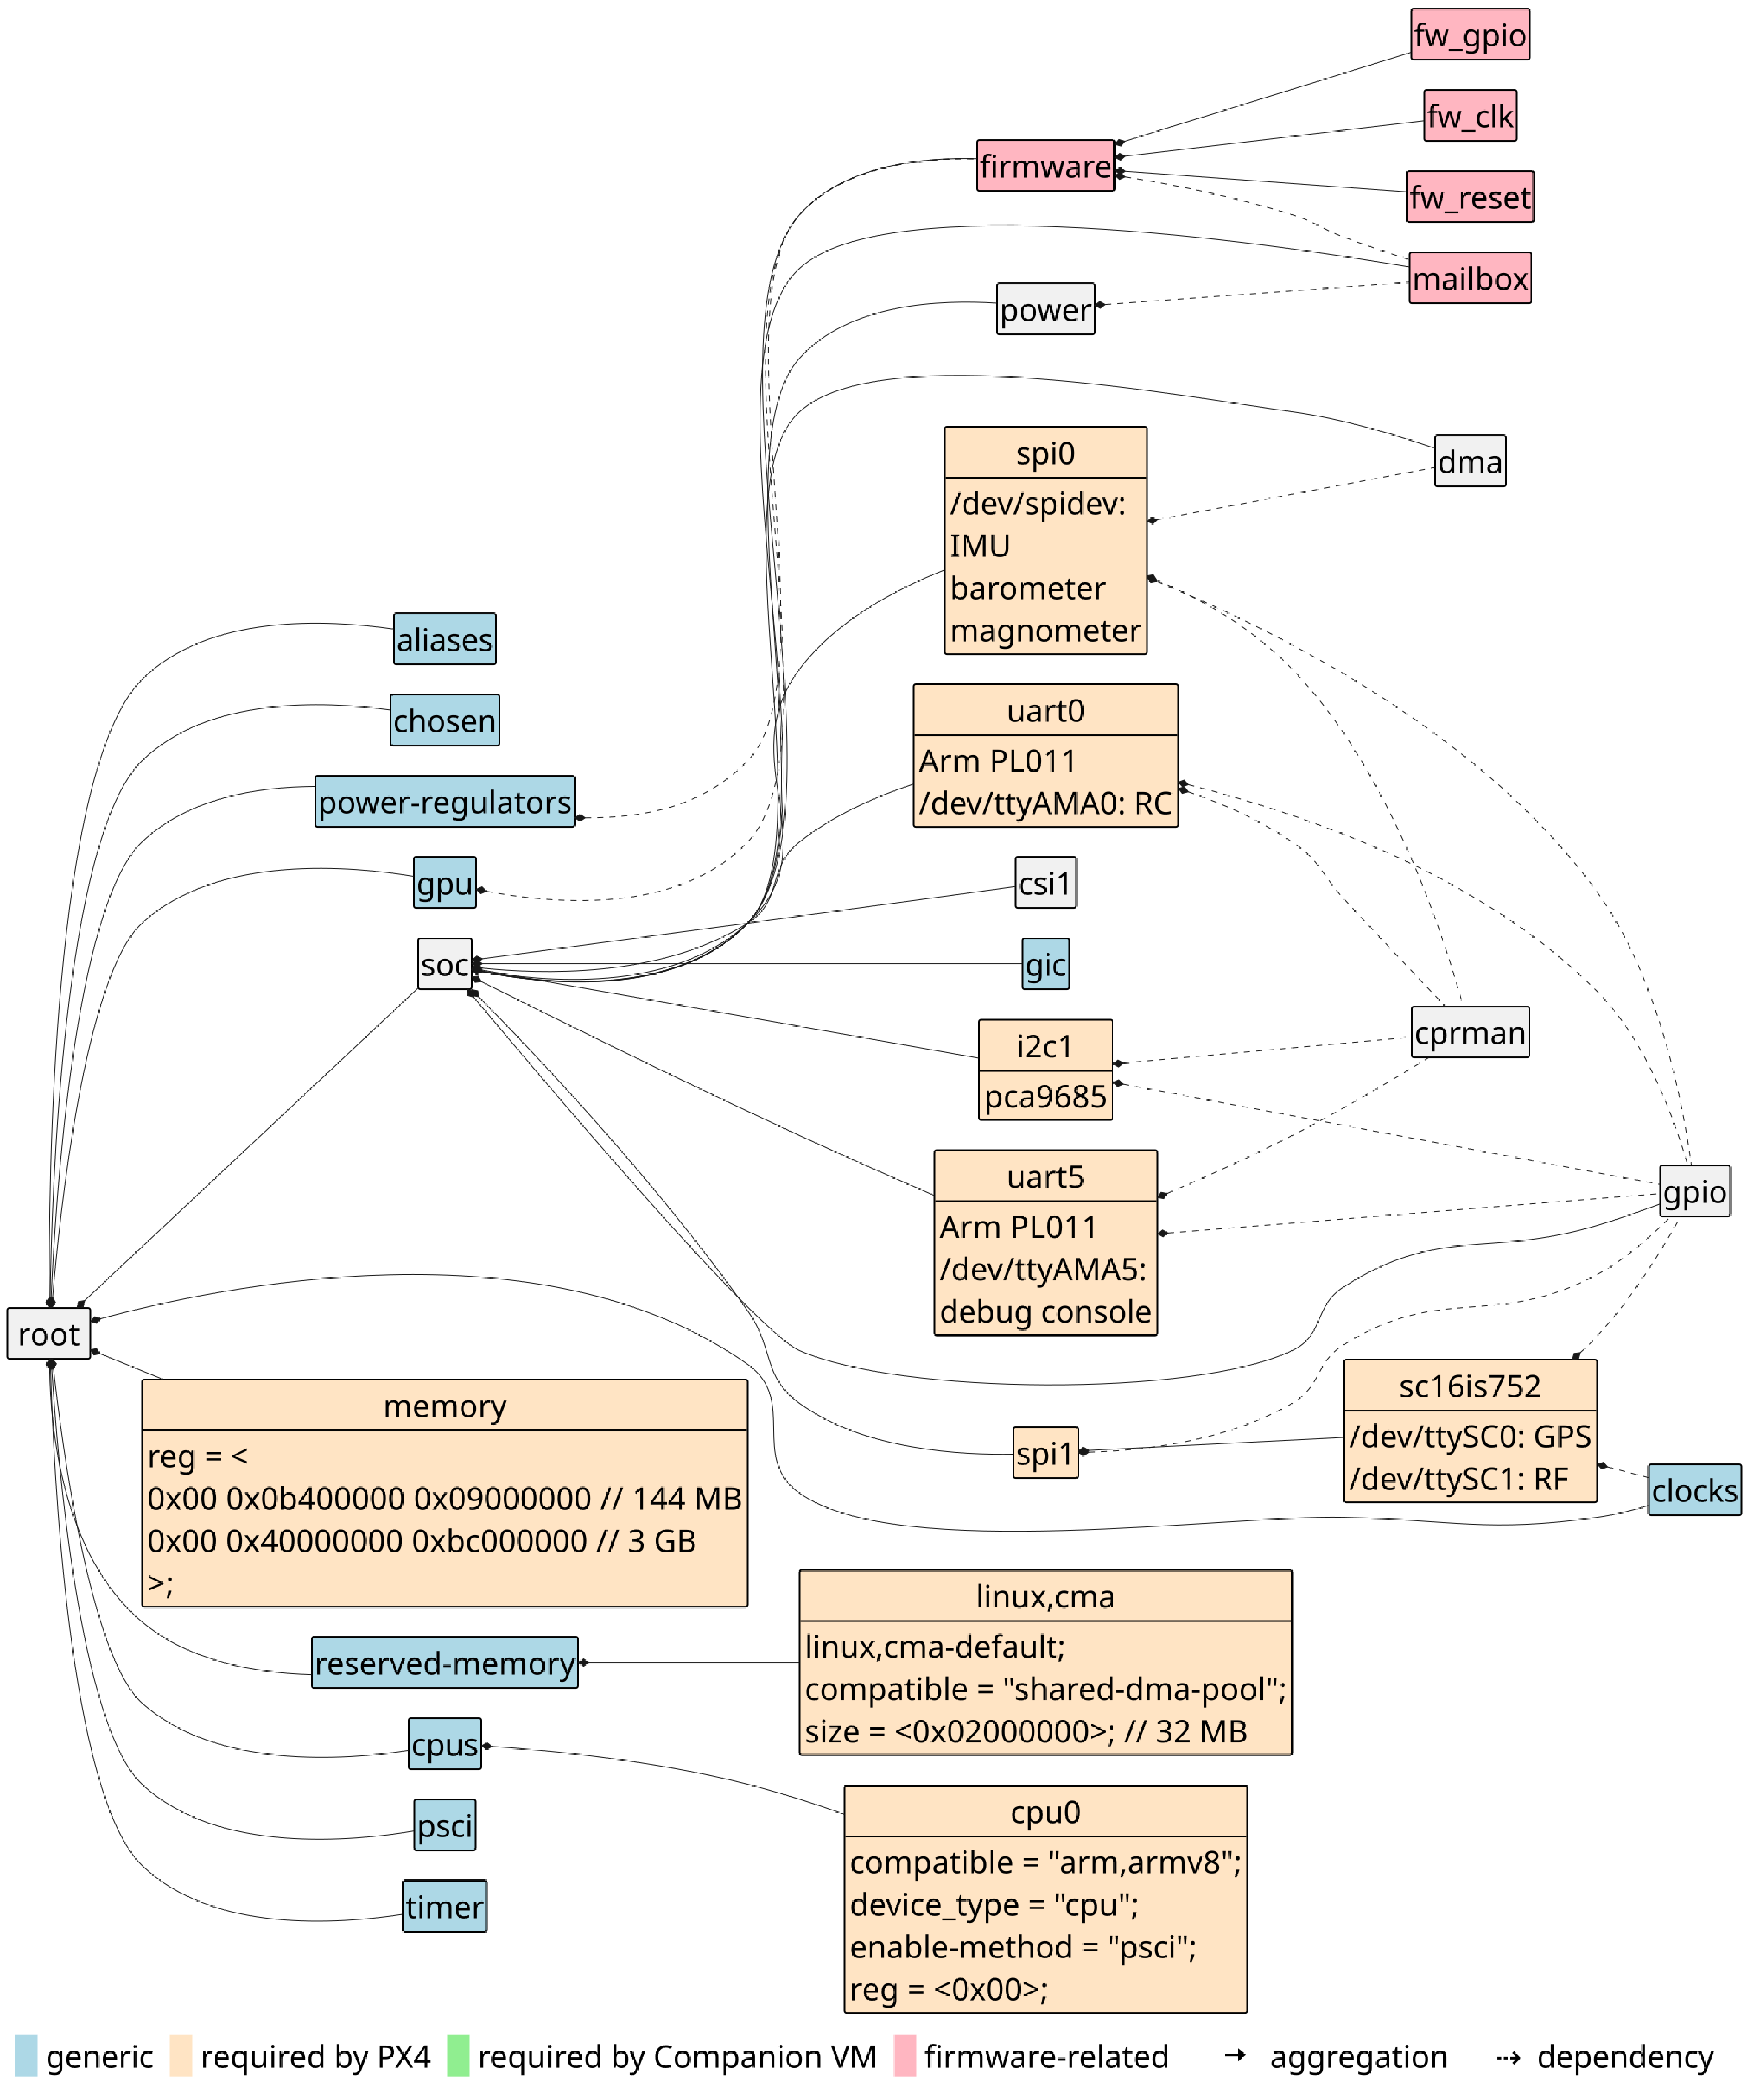
\includegraphics[width=1.0\textwidth]{./img/pdf/hw-map-2} 
  \caption[Hardware mapping: SSPFS device tree --- PX4]{Hardware mapping:
  \gls{sspfs} device tree --- PX4}%
  \label{fig:hw-map-2}
\end{figure}

\begin{figure}[!hbt]
  \centering
  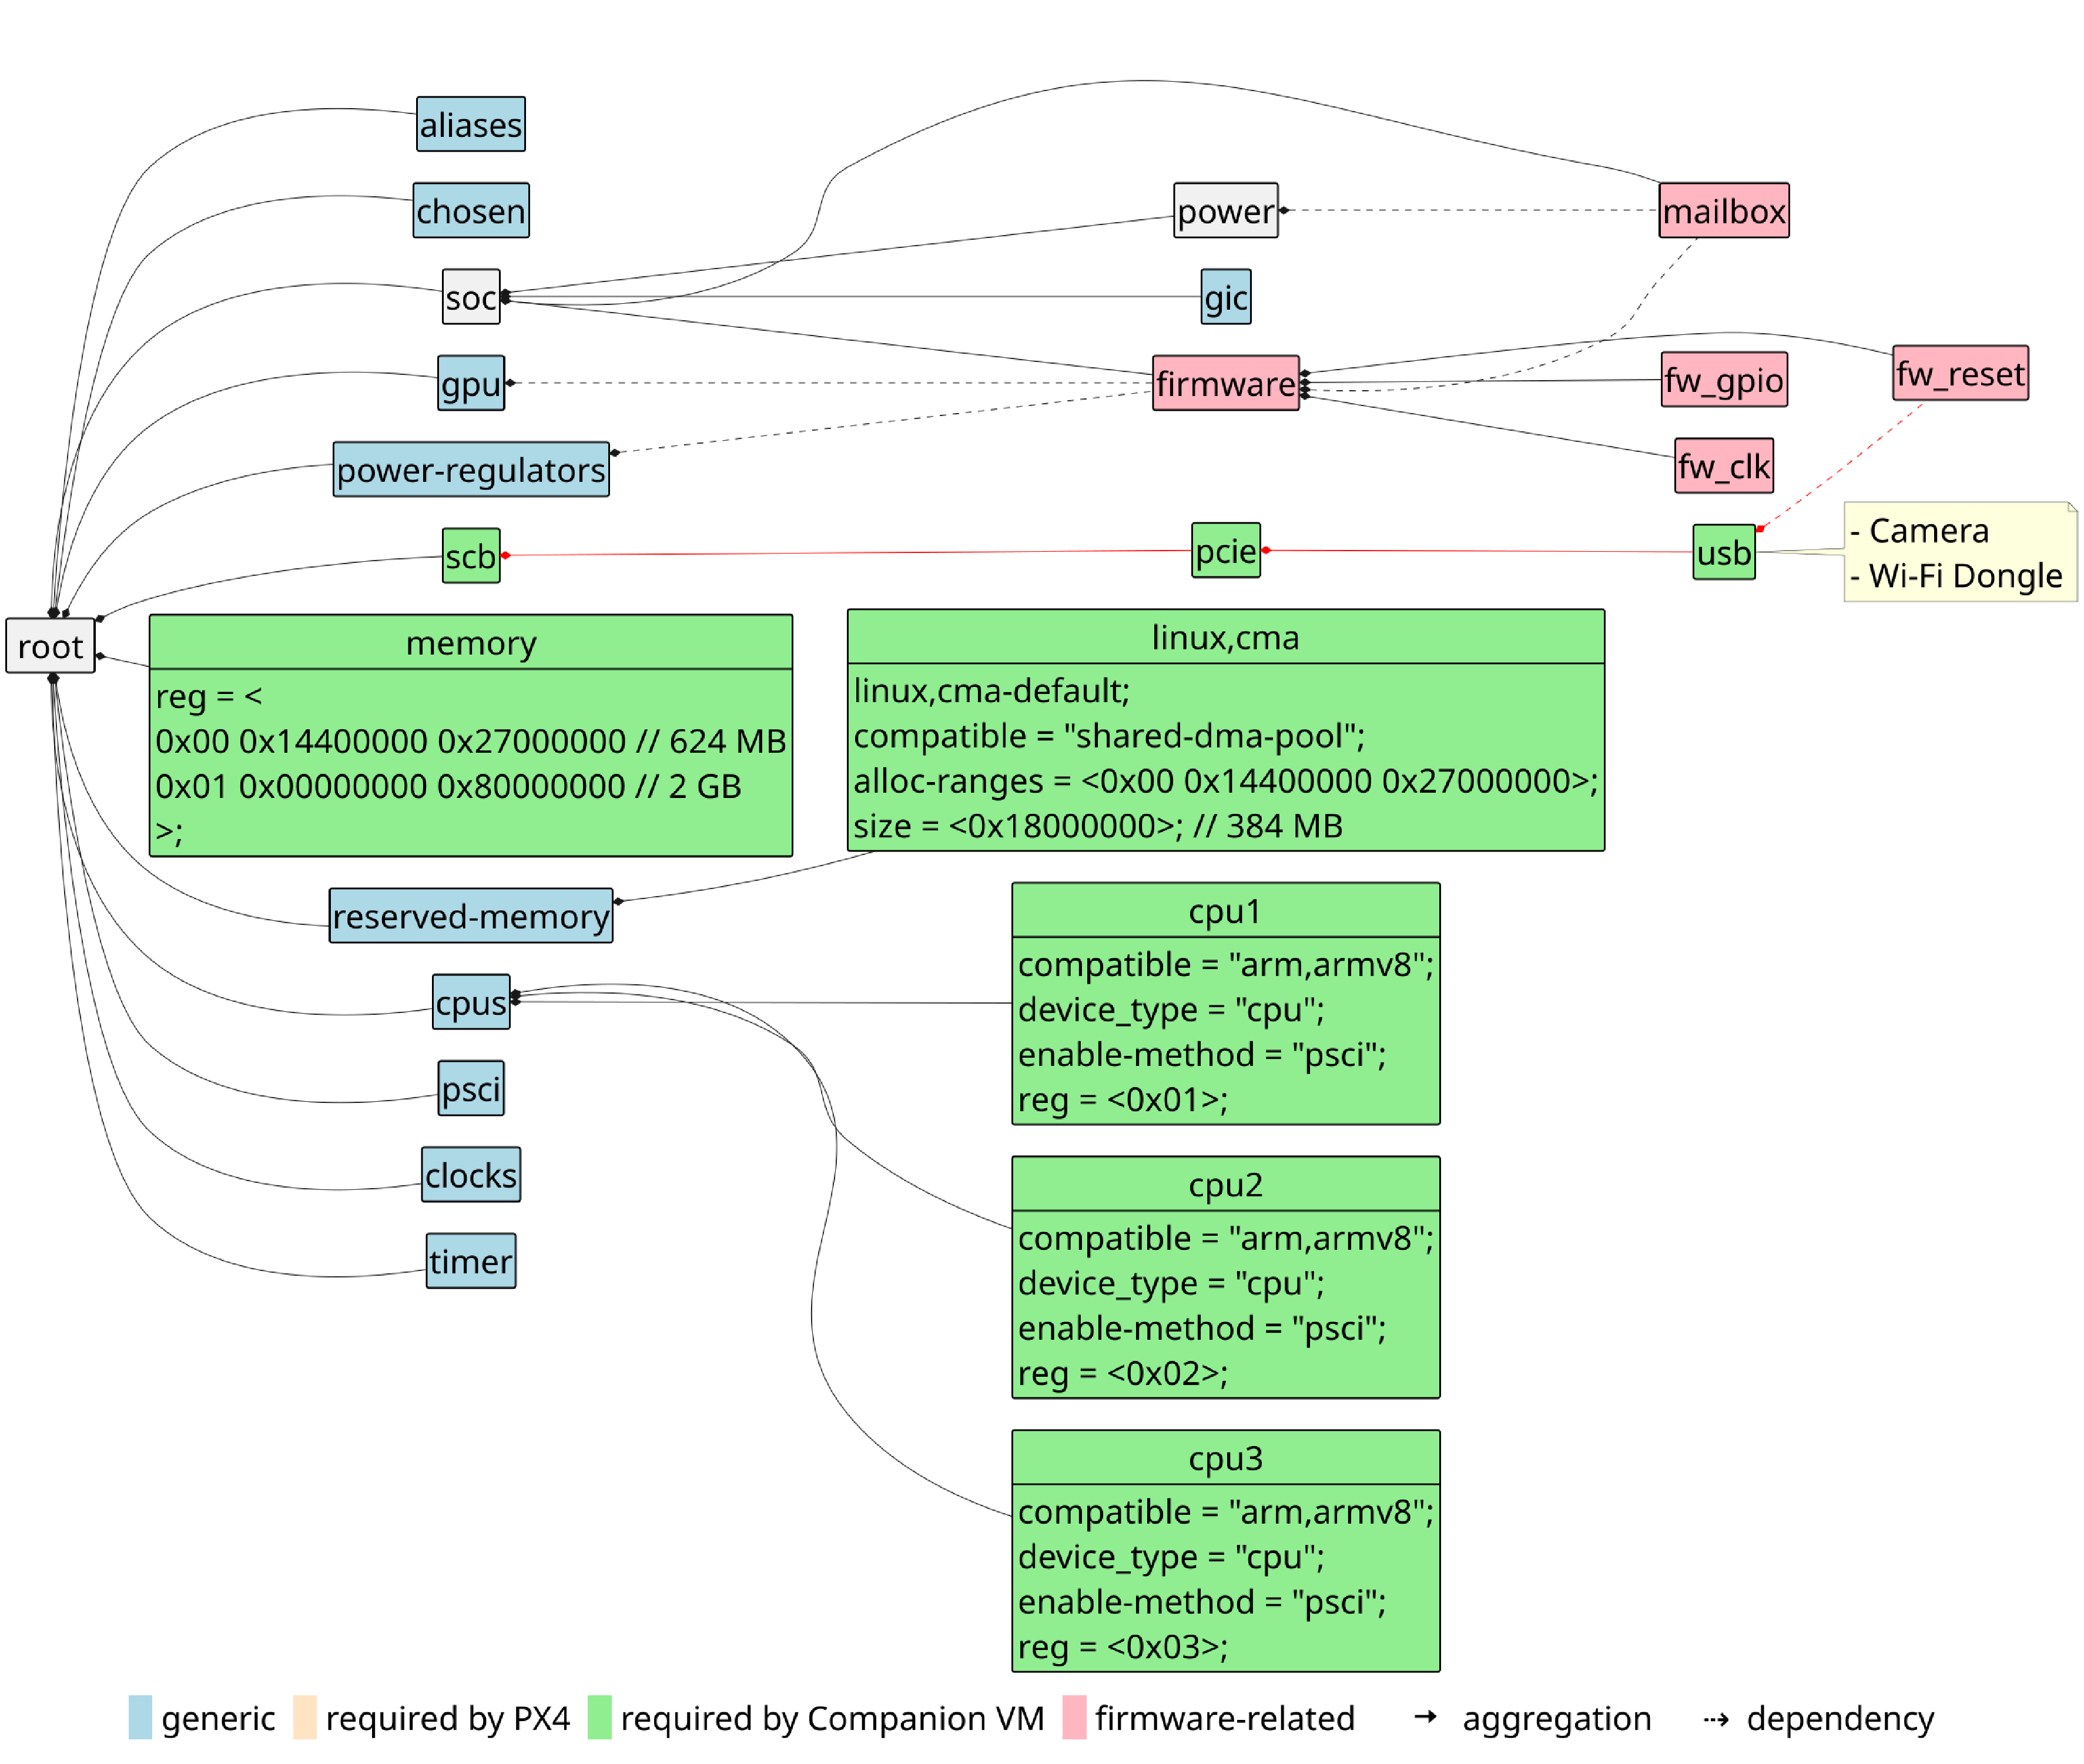
\includegraphics[width=1.0\textwidth]{./img/pdf/hw-map-3} 
  \caption[Hardware mapping: SSPFS device tree --- Companion VM]{Hardware
    mapping: \gls{sspfs} device tree --- Companion VM}%
  \label{fig:hw-map-3}
\end{figure}

The PX4 \gls{vm} includes only the required onboard
sensors/actuators and debug console (optional). Two \gls{ram} regions were
defined of 144 MB and 3 GB, respectively. From the first memory region we
reserve a \gls{cma} region of 32 MB, because the \gls{spi} devices perform \gls{dma} transactions, which is only
available in the first GB of memory~\cite{bcm2711peripherals}. Lastly, we assign one Arm
A72 \gls{cpu} (core 0).

The Companion \gls{vm} includes the \gls{usb} interface, where a \gls{usb} camera and a
\gls{usb} Wi-Fi dongle will be connected. Two \gls{ram} regions were
defined of 624 MB and 2 GB, respectively. From the first memory region we
reserve a \gls{cma} region of 384 MB, required by the video pipeline, which is only
available in the first GB of memory~\cite{bcm2711peripherals}. Lastly, we assign three Arm
A72 \glspl{cpu} (core 1--3).

\subsection{Addons}
\label{sec:addons}
The Companion \gls{vm} requires two \gls{usb} devices: a camera and Wi-Fi
dongle. Fig~\ref{fig:usb-cam} presents the selected \gls{usb} camera --- the
Creative Live! Cam Sync 1080p V2~\cite{creative-cam}.

\begin{figure}[!hbt]
  \centering
  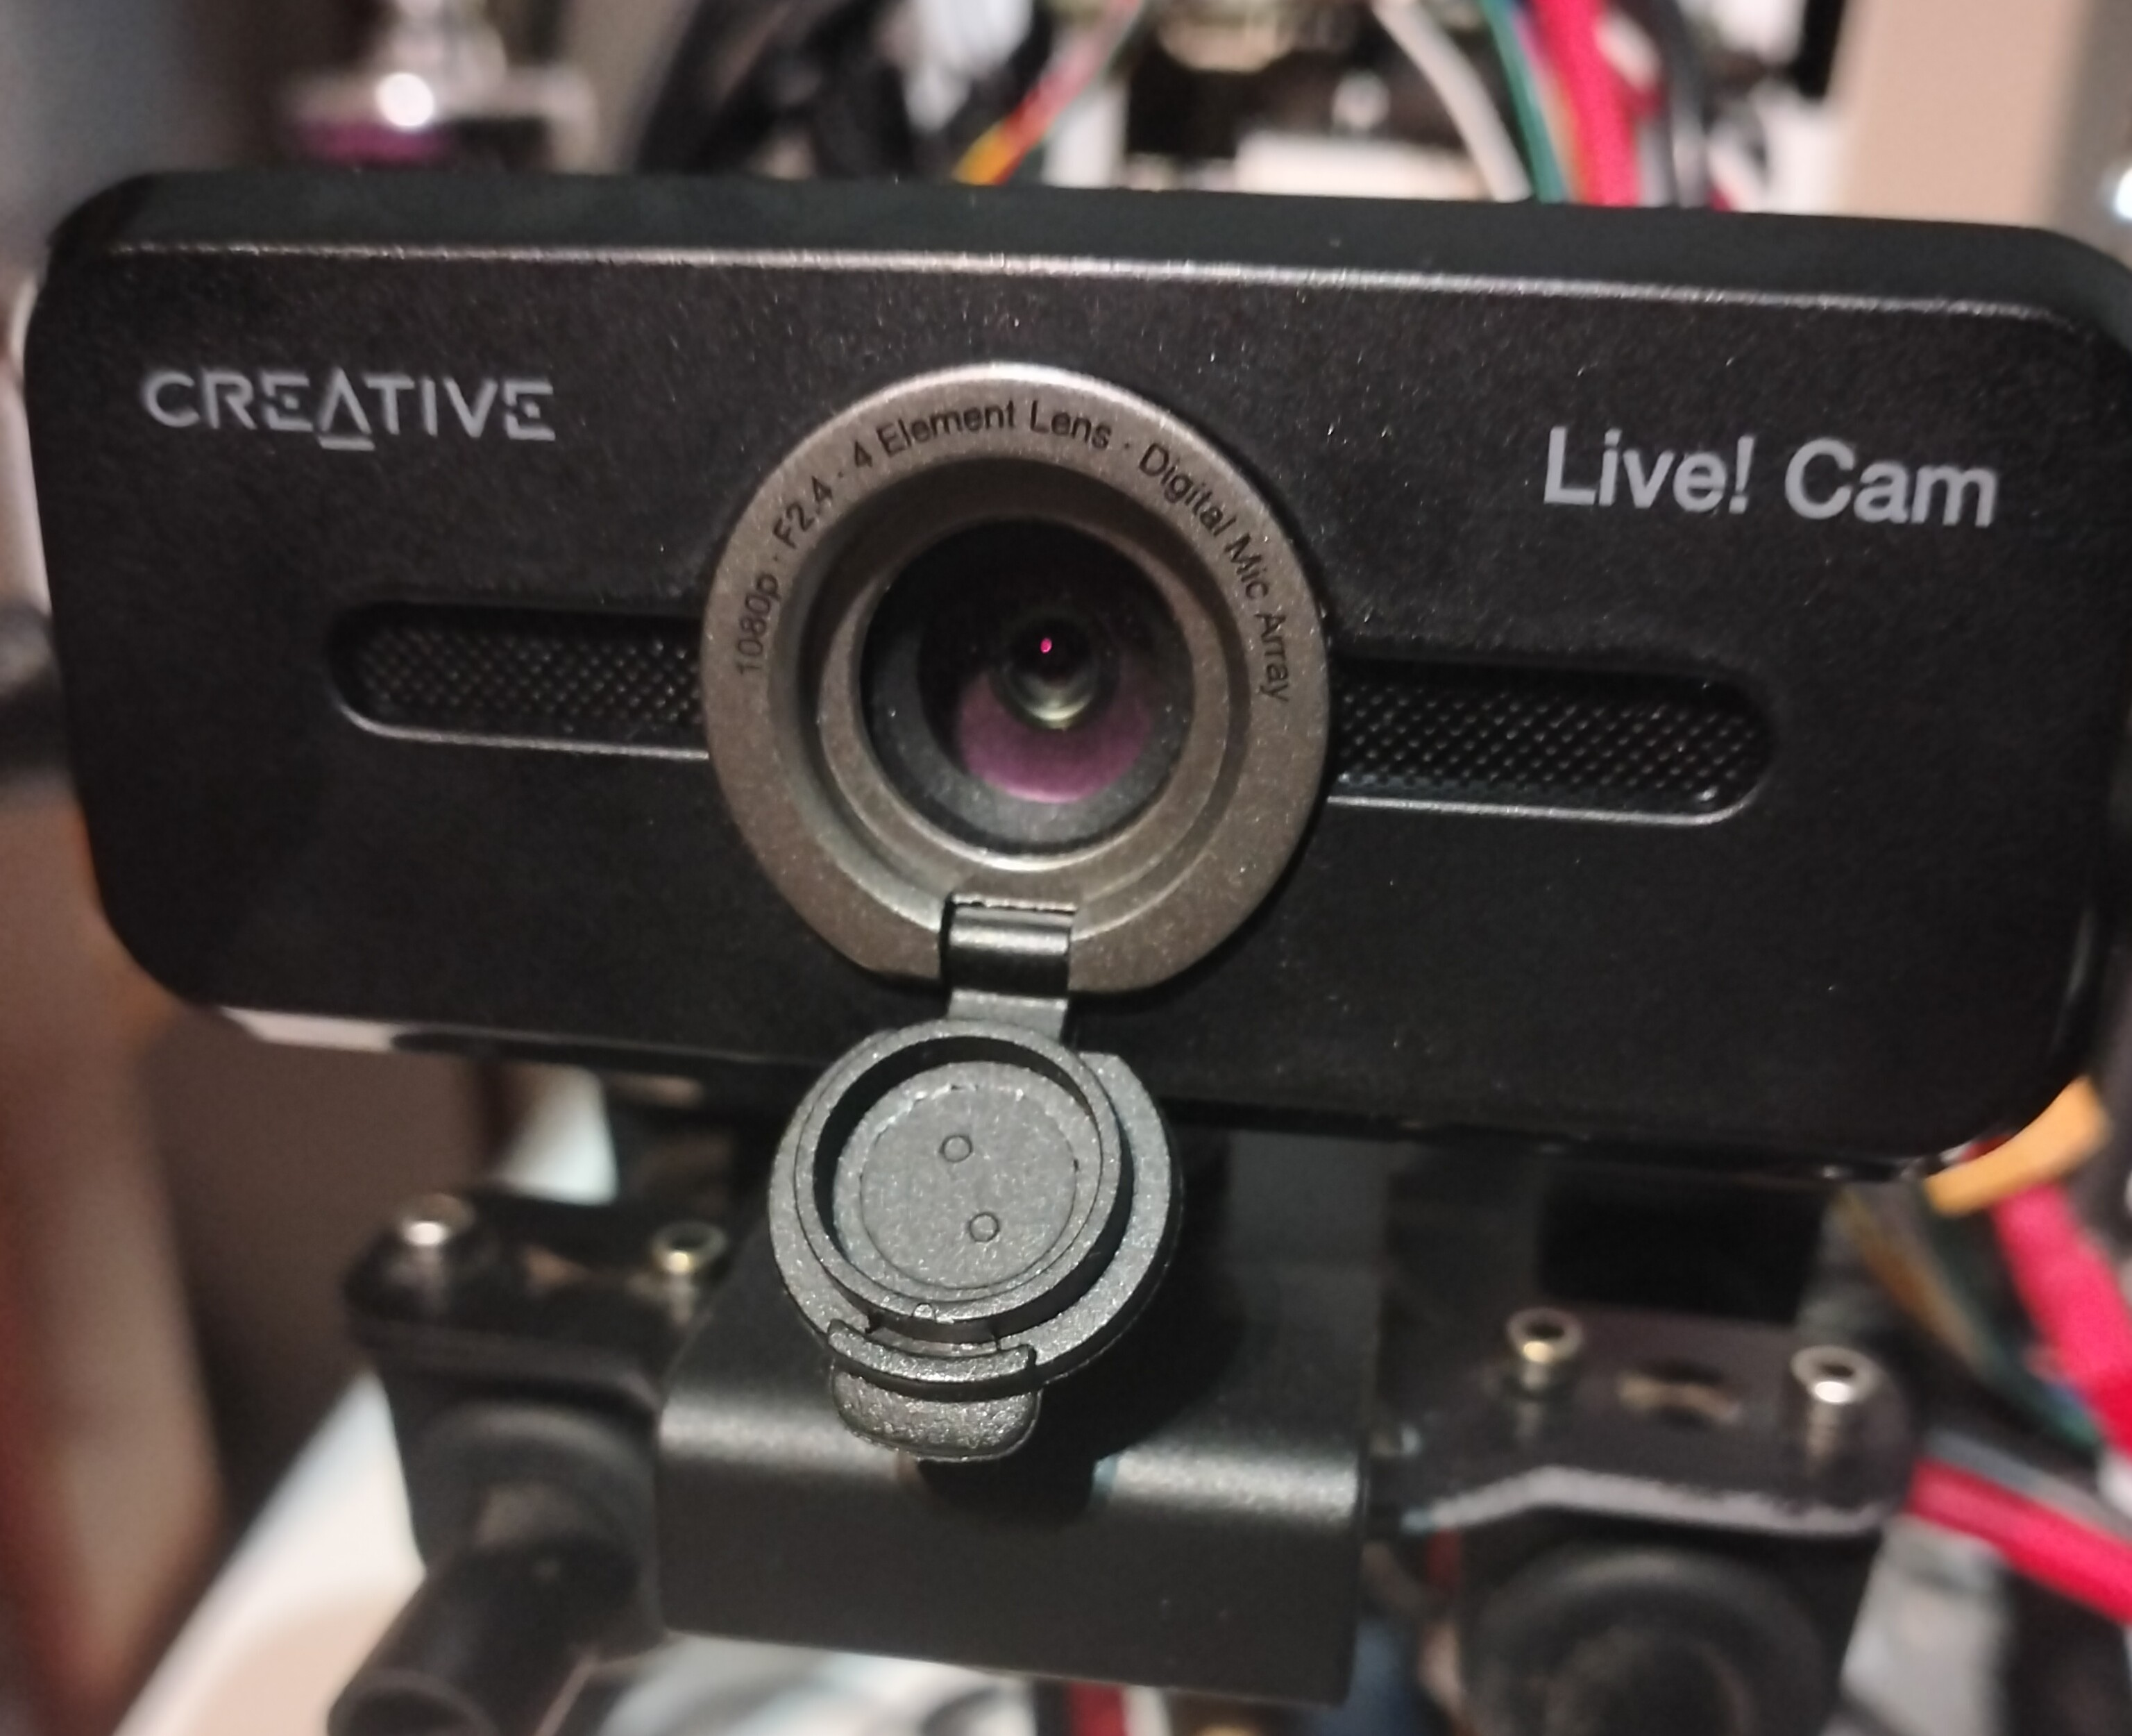
\includegraphics[width=0.5\textwidth]{./img/jpg/creative-cam} 
  \caption{Addons: USB Creative Camera}%
  \label{fig:usb-cam}
\end{figure}

It is an affordable \gls{usb} camera with full
\gls{hd} video capture (1920x1080 @ 30 \gls{fps}) and dual built-in
microphone. This camera is a plug-and-play device with built-in drivers for
Linux available out of the box. Lastly, due to its long cable it can be
positioned freely in the \gls{uav}. 

Fig.~\ref{fig:usb-wifi} presents the selected \gls{usb} Wi-Fi dongle --- the
EDUP AX3000Mbps. This dual high-gain antena device has tri-band support --- 2.4 GHz, 5, and 6
GHz --- and it can achieve data transfer rates
of up to 3000 \gls{mbps} on the \gls{usb} 3.0 interface~\cite{ax3000-specs}. It contains a Mediatek
\texttt{mt7921au} chipset with a wide \gls{os} compatibility, supported
in-kernel since Linux kernel 5.18~\cite{ax3000-linux}.

\begin{figure}[!hbt]
  \centering
  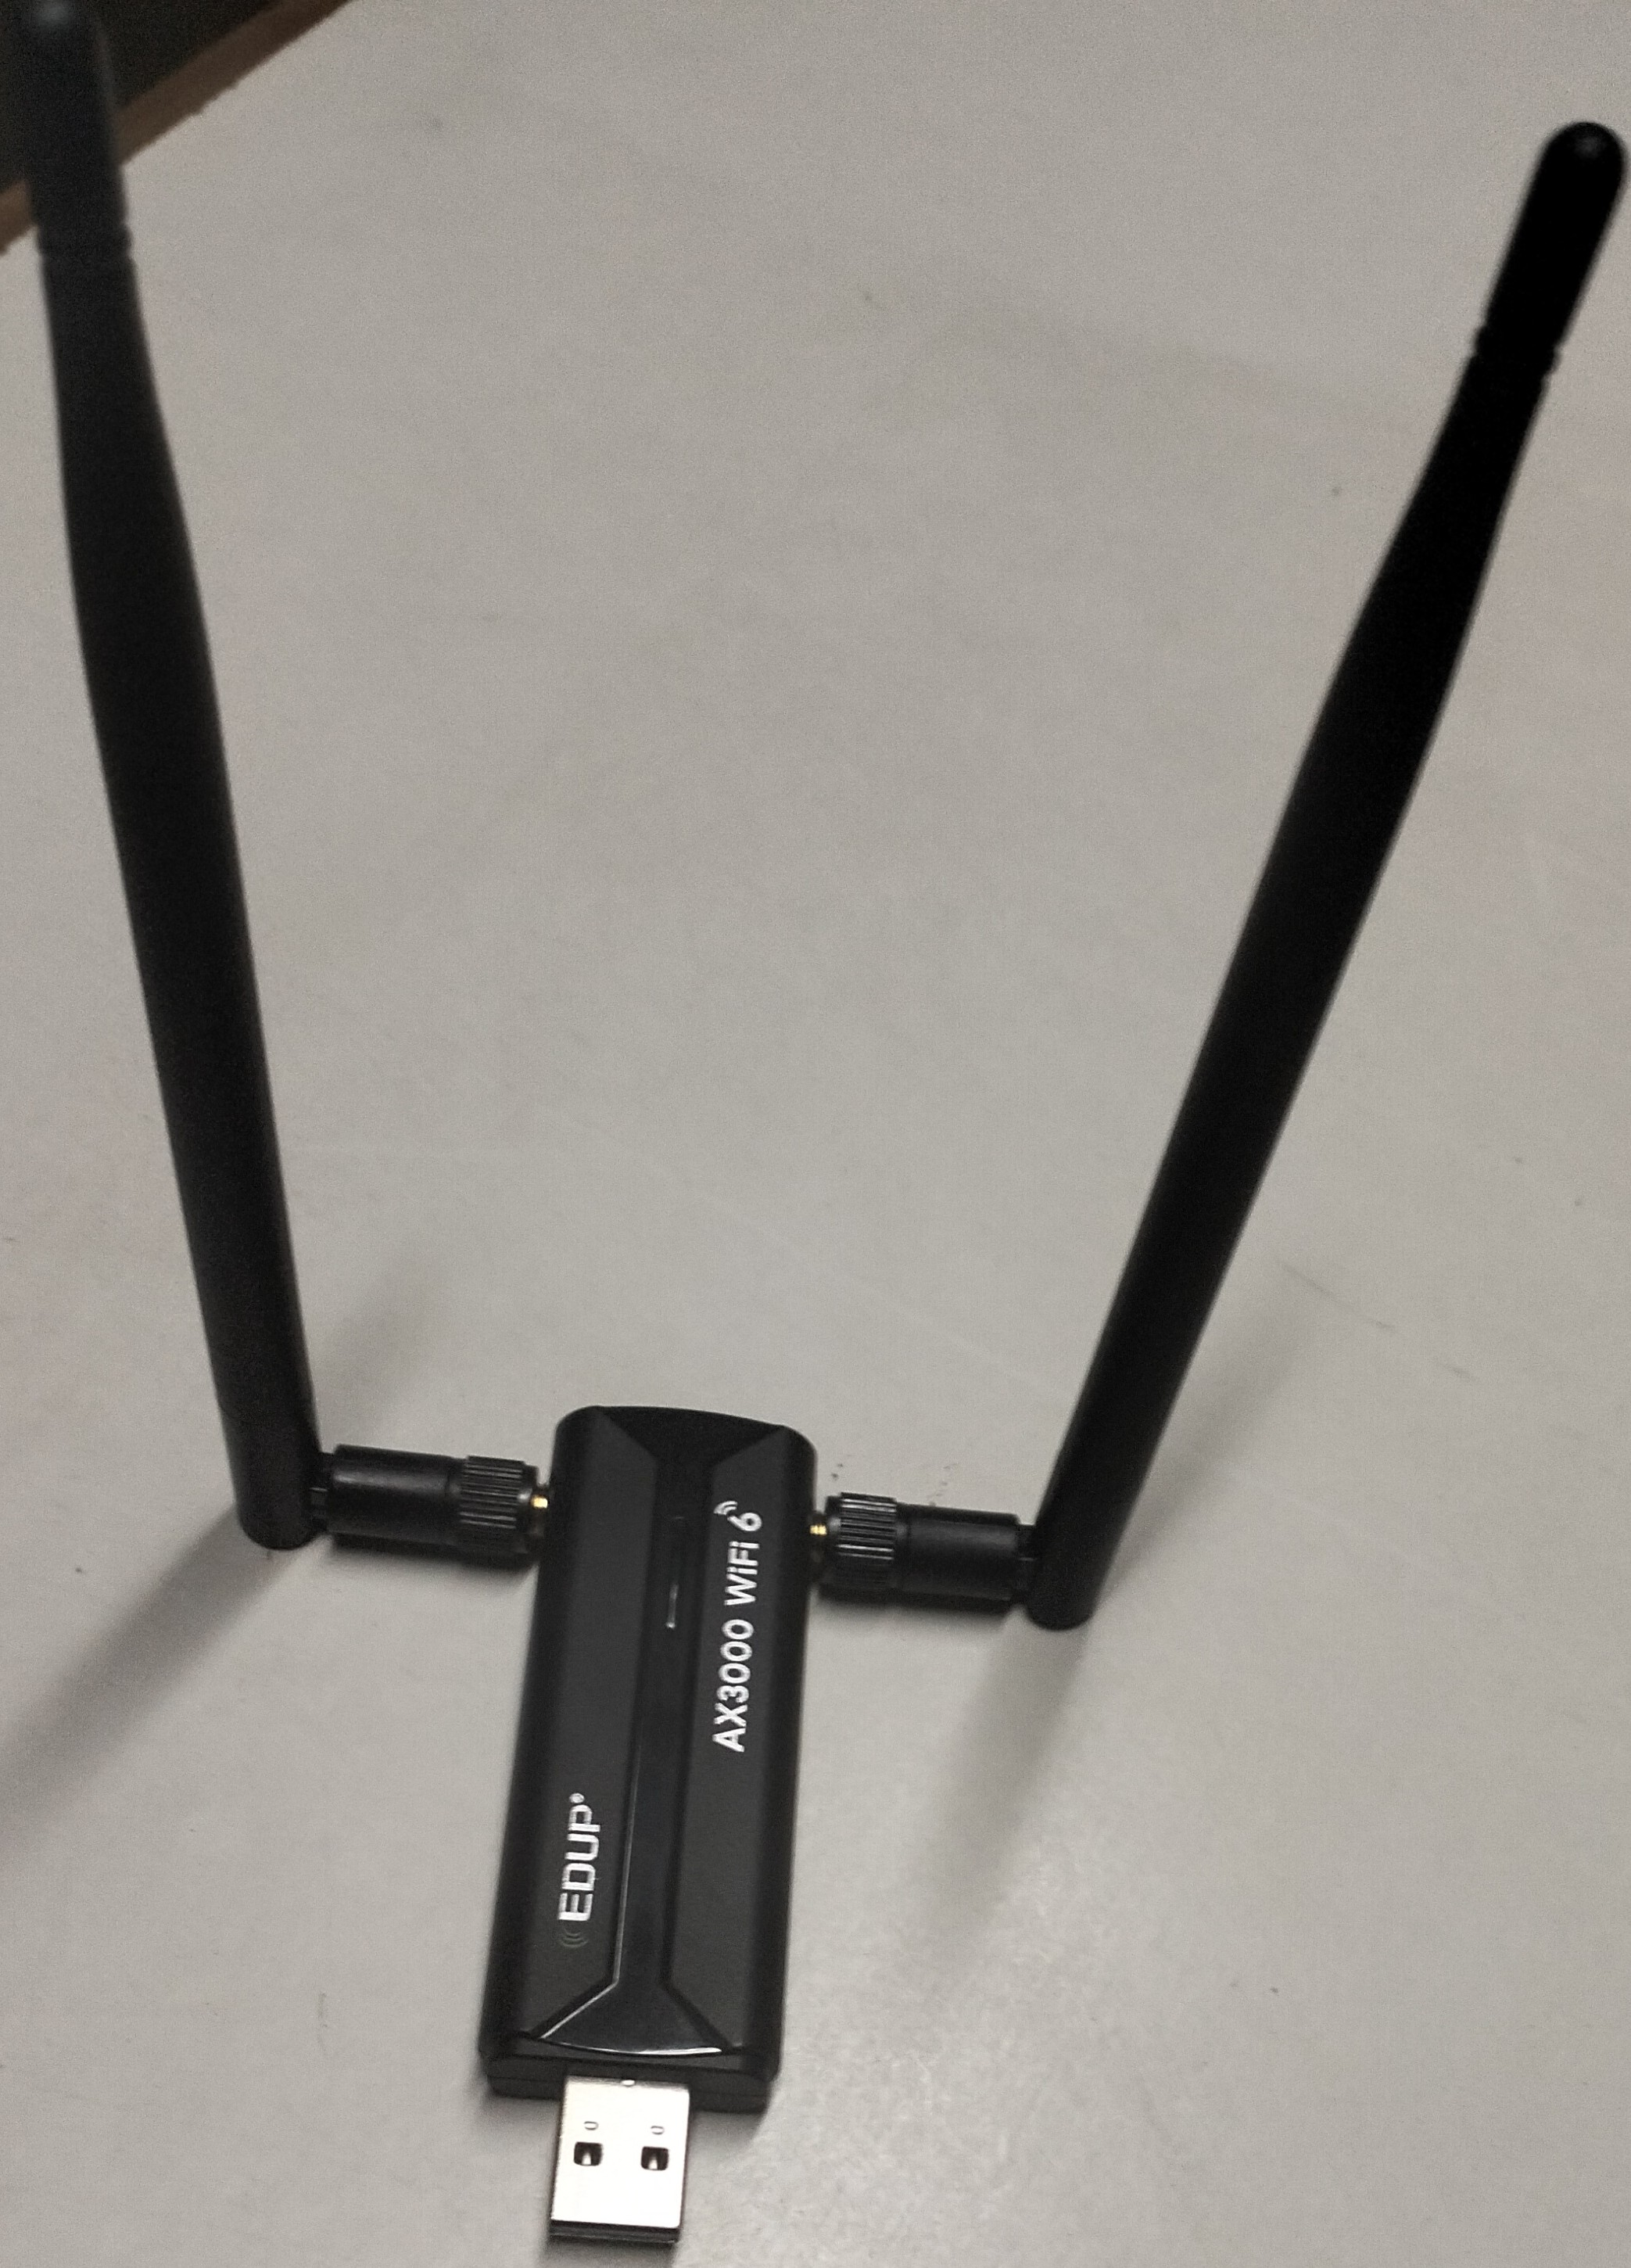
\includegraphics[width=0.4\textwidth]{./img/jpg/ax3000} 
  \caption{Addons: USB Wi-Fi dongle --- EDUP AX3000}%
  \label{fig:usb-wifi}
\end{figure}


%%% Local Variables:
%%% mode: latex
%%% TeX-master: "../template"
%%% reftex-default-bibliography: ("../Bibliography/mieeic.bib")
%%% ispell-local-dictionary: "american"
%%% End:
